\documentclass[12pt]{report}
\usepackage[utf8]{inputenc}
\usepackage[english]{babel}
\usepackage{microtype}
\usepackage{libertine}
\usepackage{amsmath,amsthm}
\usepackage[varg]{newtxmath}
\usepackage{setspace,graphicx,epstopdf}
\usepackage{marginnote,datetime,url,enumitem,subfigure,rotating}
\usepackage{multirow}
\usepackage{xfrac}
\usepackage[openlevel=3]{bookmark}
\usepackage[tikz]{bclogo}
\usepackage{enumitem}

\setcounter{tocdepth}{2}

\def\D{\mathrm{d}}

\setlength{\parindent}{0ex}
\setlength{\parskip}{1em}%Espacement des par

\setlist[itemize]{topsep=-5pt,itemsep=0pt}

\newtheorem{theorem}{Theorem}[chapter]
\newtheorem{definition}{Definition}[chapter]
\newtheorem{assumption}{Assumption}[chapter]
\newtheorem{proposition}{Proposition}[chapter]

\newcommand{\E}[1]{\operatorname{E}\left[#1\right]}
\newcommand{\Et}[1]{\operatorname{E}_t\left[#1\right]}
\newcommand{\V}[1]{\operatorname{Var}\left[#1\right]}
\newcommand{\cov}[1]{\operatorname{Cov}\left(#1\right)}
\newcommand{\avg}[2]{\frac{#1}{#2} \sum_{i=#1}^{#2}}

\begin{document}

\date{}
\title{ECON7750 - Macroeconomic Th. I\\ Lecture Notes}
\author{Paul Anthony Sarkis\\ Graduate Student in Economics \\Boston College} 
 
\maketitle

\tableofcontents


\chapter{Solow Growth Model}

The objective of this chapter is to design a simple framework (model) identifying proximate causes of growth as well as its mechanisms. The Solow-Swan model (named after Bob Solow and Trevor Swan) comes after the previously most common model: the Harrod-Domar model. The HD model emphasized on dysfunctional aspects of growth like unemployment. The Solow model demonstrates why HD is not satisfying as growth model go. We find the neoclassical production function in the latter.

\section{Assumptions}

\subsection{Inputs and Outputs}

We will see that the Solow model is interested in the behavior of four main variables, namely output($Y$), capital ($K$), labor ($L$) and "knowledge" ($A$). The three last variables are going to produce output through a process called production, represented by the following function: $$Y(t) = F[K(t), A(t)\cdot L(t)] $$ Already, there are quite a few elements to notice. First, all inputs and output are time-varying but the production function is not (the function $F$). This means that output will change over time if and only if inputs vary. Second, notice that knowledge and labor inputs interact with each other. This implies that the level of knowledge allows for a higher input of labor, even if $L$ did not change. Because it affects efficiency of labor, we will call $AL$ the effective labor. This type of knowledge is called labor-augmenting knowledge or Harrod-neutral. We will see later why this assumption is so important in the Solow model.

\subsection{Production Function}

\begin{assumption}[Continuity, Differentiability, Positive and Diminishing Marginal Products and CRS]
Let $F:\mathbb{R}^3\to\mathbb{R}$ be the production function. We assume that $F$ is twice continuously differentiable in $K$ and $AL$ such that:\begin{itemize}
\item The MP of K is positive and diminishing: $F_K > 0$ and $F_{KK} < 0$.
\item The MP of AL is positive and diminishing: $F_L > 0$ and $F_{LL} < 0$.
\end{itemize} Further, we assume that $F$ is homogeneous of degree 1 and hence displays constant returns to scale.
\end{assumption}

The last assumption of constant returns to scale can be given two main rationale. First, this implies that the economy is already mature and that gains from specializing are all exhausted already. Second, the inputs will always be used in the same way (in the same production function) regardless of the amount. We can use the homogeneity of the function to modify the function a bit: $$Y = F[K, AL] \Leftrightarrow \frac{Y}{AL} = F\left[\frac{K}{AL}, 1\right] $$ We denote all variables divided by $AL$ by their uncapitalized counterparts: $y\equiv Y/AL$ and so on. Because $AL$ is efficient labor, we call $y$ and $k$ the variables "per unit of effective labor". We also define $f(k)\equiv F\left[K/AL, 1\right] $, the intensive form of the production function. From that new form, we can get new forms for the input derivatives: \begin{itemize}
\item $\frac{\partial}{\partial K}F[K, AL] = \frac{\partial}{\partial K}(ALf(k)) = f'(k)$
\item $\frac{\partial}{\partial AL}F[K, AL] = \frac{\partial}{\partial K}(ALf(k)) = f(k) - AL\frac{K}{(AL)^2}f'(k) = f(k) - kf'(k) $
\end{itemize}

\begin{theorem}[Euler's theorem]
Let $f:\mathbb{R}^{K+2}\to\mathbb{R}$ be continuously differentiable in $x$ and $y$ and is homogeneous of degree $m$. Then, $$m g(x,y,\cdot) = x\cdot g_x(x,y,\cdot) + y\cdot g_y(x,y,\cdot) \quad \forall x,y\in\mathbb{R}\text{ and }z\in\mathbb{R}^K $$ Moreover, $g_x$ and $g_y$ are both homogeneous of degree $m-1$ in $x$ and $y$.
\end{theorem}

\begin{assumption}[Inada conditions]
Let $F:\mathbb{R}^3\to\mathbb{R}$ be the production function. We assume that:$$ \lim_{K\to 0} F_K = \infty\text{ and }\lim_{K\to\infty} F_K = 0 $$
$$ \lim_{L\to 0} F_L = \infty\text{ and }\lim_{L\to\infty} F_L = 0$$
\end{assumption}

\subsection{Evolution of Inputs}

Finally, just before going to solving the model, we'll need to define how our inputs are going to move in time. We'll assume that labor and knowledge grow at constant rates: $$\frac{\dot{L}(t)}{L(t)} = n \text{ and } \frac{\dot{A}(t)}{A(t)} = g $$ where $n$ and $g$ are exogenous parameters of our model.

For capital, we'll include a slightly more complex dynamics. We'll assume that the variation in capital is determined by new investment and depreciation of existing capital such that: $$\dot{K} = I - \delta K$$ Here $\delta$ is an exogenous parameter as well and we'll define investment to be a exogenously fixed proportion of total output, denoted $s$. Hence, it is as if consumers getting $Y$ as income choose to save a proportion $s$ of this income and invest it in the formation of new capital stock. Finally, $$\dot{K} = sY - \delta K$$

\section{Solving the model}

Now that we have described how inputs interact with output in a static way, we ask how this interaction will change over time. We already know that labor and input are dynamically fixed, however capital is not, it will therefore be our main object of study.

\subsection{Dynamics of $k$}

Recall that the stock of capital moves according to $\dot{K} = sY - \delta K$ but it turns out it will be much easier to analyze the behavior of capital per unit of effective labor, $k$. By the chain rule: \begin{align*} k = K/AL \Leftrightarrow \dot{k} =  \frac{\dot{K}(AL) - [\dot{A}L + A\dot{L}]K}{(AL)^2} & \Leftrightarrow \dot{k}  =  \frac{\dot{K}}{AL} - \frac{[\dot{A}L + A\dot{L}]}{AL}\frac{K}{AL} \\
& \Leftrightarrow \dot{k}  =  \frac{sY - \delta K}{AL} - (n + g)k \\
& \Leftrightarrow \dot{k}  =  sy - (\delta + n + g)k\\
& \Leftrightarrow \dot{k}  =  sf(k) - (\delta + n + g)k
\end{align*} This equation is the key to solving the Solow model. We can interpret it as a description of the rate of change of capital stock per unit of effective labor: $sf(k)$ is investment per unit of effective labor while $(n+g+\delta)k$ is the effective depreciation. In order to keep the capital stock per unit of effective labor from falling, we must invest $(n+g+\delta)k$.

We can represent the situation in two graphs. First, if we represent investment as a function of capital we get the following graph:\begin{center}
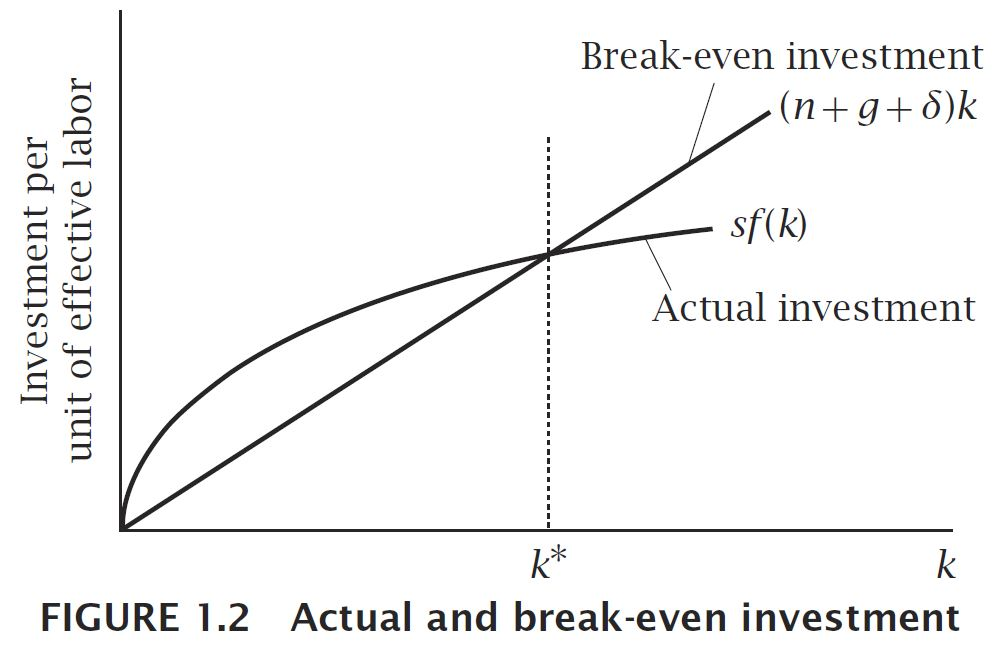
\includegraphics[scale=0.33]{images/Solowbreakeven}
\end{center}

The second graph is the phase diagram, plotting the variation of $k$ with respect to its own level:
 
\begin{center}
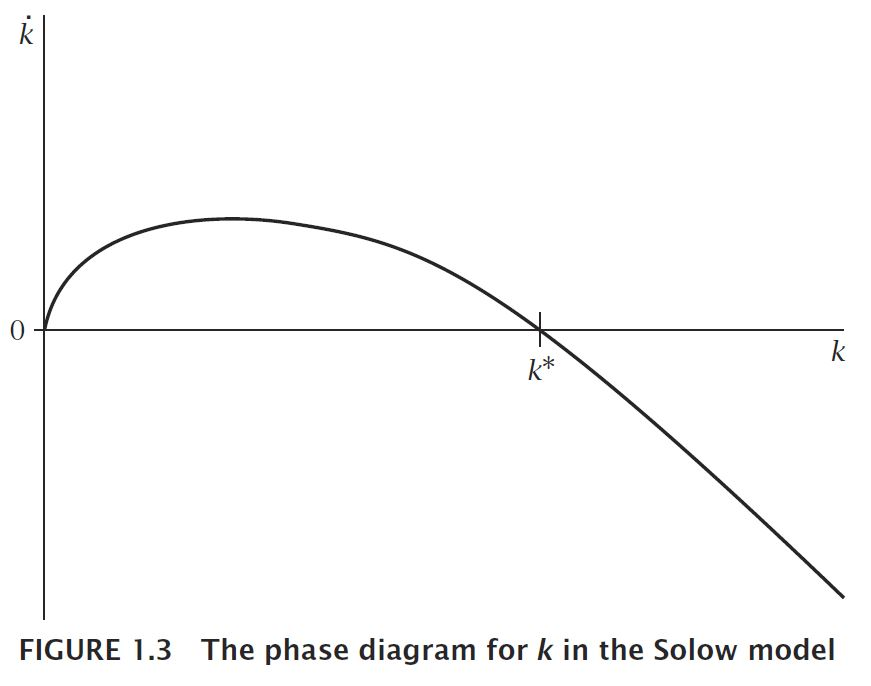
\includegraphics[scale=0.35]{images/Solowphase}
\end{center}

\subsection{Balanced growth path}

We can now solve for the balanced growth path where $\dot{k} = 0$. This gives: $$sf(k^*) = (\delta + n + g)k^* \Leftrightarrow f(k^*)/k^* = (\delta + n + g)/s $$ With a specification for $f(k)$ we could actually solve this model easily. Nevertheless, without even specifying it we can still say quite a lot about the dynamics of our model. To do that, recall that $L$ and $A$ grow at rates of $n$ and $g$ respectively. Therefore:\begin{itemize}
\item $K = ALk \Leftrightarrow \dot{K} = k(\dot{A}L + \dot{L}A) \Leftrightarrow \dot{K}/K = \dot{A}/A + \dot{L}/L = n + g $
\item $\dot{Y}/Y = n + g$ because of CRS (and inputs grow at that rate).
\item $\dot{C}/C = n + g$ because $C = (1 -s)Y$.
\item We can deduce that all per worker variables will grow at rate $g$.
\end{itemize}

\section{Impact of a change in $s$}

The parameter of the Solow model that policy is the most likely to affect is $s$. Indeed, because government behavior will affect people's propensity to save, we'll study the effects of variations in $s$ closely. All dynamic results of an increase in the savings rate will be presented in the end of the chapter.

\subsection{Impact on output}

We know that an increase in $s$ will cause an increase in $sy(t)$ and hence the break-even point $k^*$ will shift to the right to $k^{*'}$ (i.e. the optimal capital stock per unit of effective labor will increase). However, $k$ did not change immediately and is still at the previous equilibrium point. At this level, we have that $sf(k) > (\delta + n + g)k$ and hence $\dot{k} > 0$ until $k = k^{*'}$.

What happens to output per worker, $Y/L$? On the balanced growth path, output per worker grows at rate $g$. When $s$ increases, we have seen that it implies a hike in the growth rate of $k$ and hence on $K$ as well as $Y$. Therefore, the growth rate of $Y/L$ will increase temporarily, as long as $\dot{k}>$ and then return to $g$.

\subsection{Impact on consumption}

From the national income accounting, we know that $C = Y - I$ and hence we also have $c(t) = y(t) - i(t)$. Moreover, on the BGP, we have also that $y(t) = f(k^*)$ and $i(t) = sf(k^*) = (\delta + n +g)k^*$. Therefore, $$c^* = f(k^*) - (n+g+\delta)k^*$$ and differentiating by $s$ gives us: $$\frac{\partial c^*}{\partial s} = f'(k^*) - (\delta + n +g)\frac{\partial k^*}{\partial s} $$ It is clear that the result of this depends on the magnitude of $f'(k^*)$. The intuition behind this is that increasing the savings rate will lead to a higher optimal capital: does this higher capital stock produces more output than it needs maintenance? If yes, then the additional output will serve to consume more. If not, consumption will have to decrease as a result.

Another interesting intuition from this last equation is that there must exist a level of $s$ such that $k^*$ makes $\frac{\partial c^*}{\partial s} = 0$ implying that consumption per unit of effective labor is at its maximum. This value of $k^*$ is known as the golden-rule level of capital stock, denoted by $k^G$.

\begin{center}
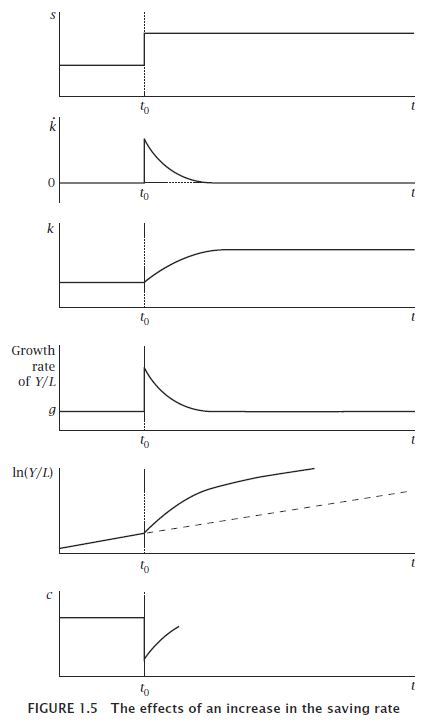
\includegraphics[scale=0.75]{images/solowsshock}
\end{center}

\section{Quantitative Implications}

In this section we will present the quantitative results that will allow us to estimate and compare the Solow model results to actual observations. We'll look into the effect of the savings rate on the output as well as the speed of convergence to the steady state.

\subsection{Effect on Output in the Long Run}

We know that output on the BGP is given by: $$y^* = f(k^*)$$ and hence, $$\frac{\partial y^*}{\partial s} = f'(k^*)\cdot \frac{\partial k^*}{\partial s} $$ The two parts of this derivative will need to be found.

The optimal level of capital $k^*$ is intrinsically determined by the condition $\dot{k} = 0$, therefore it must be that $sf(k^*) = (n+g+\delta)k^*$ and when you differentiate with respect to $s$ you get: $$sf'(k^*)\frac{\partial k^*}{\partial s} + f(k^*) = (n+g+\delta)\frac{\partial k^*}{\partial s} $$ and therefore we can find $$\frac{\partial k^*}{\partial s} = \frac{f(k^*)}{(n + g + \delta) - sf'(k^*)} $$ which finally gives: $$ \frac{\partial y^*}{\partial s} = \frac{f'(k^*)\cdot f(k^*)}{(n + g + \delta) - sf'(k^*)} $$

In order to ease the interpretation of this very complex equation, we'll transform it into an elasticity by multiplying both sides by $s/y^*$. $$\frac{\partial y^*}{\partial s}\frac{s}{y^*} = \frac{s}{f(k^*)}\cdot \frac{f'(k^*)\cdot f(k^*)}{(n + g + \delta) - sf'(k^*)} = \frac{sf(k^*)\cdot f'(k^*)}{f(k^*)\cdot[(n + g + \delta) - sf'(k^*)]} $$ We know that $sf(k^*) = (n+g+\delta)k^*$, therefore: $$ \frac{\partial y^*}{\partial s}\frac{s}{y^*} = \frac{(n+g+\delta)k^* \cdot f'(k^*)}{f(k^*)\cdot[(n + g + \delta) - (n + g + \delta)\cdot (k^*/f(k^*))]} = \frac{k^* f'(k^*)/f(k^*)}{1 - (k^*f'(k^*)/f(k^*))}$$ where $(k^*f'(k^*)/f(k^*))$ is the elasticity of capital input in the production function, denote it $\alpha_K$.

How can we interpret the last result: $\frac{\partial y^*}{\partial s}\frac{s}{y^*} = \frac{\alpha_K(k^*)}{1 - \alpha_K(k^*)}$? First, we must notice that in competitive markets, capital must earn it marginal product $f'(k)$ (firm optimization under perfect competition). Thus, the total amount earned by capital on the BGP is $k^*f'(k^*)$ (quantity $\times$ price), and the share of total income that comes from capital is $(k^*f'(k^*))/y^* = (k^*f'(k^*))/f(k^*) = \alpha_K(k^*)$. This result is very important because it allows us to estimate the elasticity of capital in the production function using the capital share of income! Second, using $\alpha_K(k^*) = 1/3$, we can estimate the savings-elasticity of output to be a half on the BGP, meaning that a $10\%$ increase in the savings rate will lead to an long-run increase of $5\%$ in the output per unit of effective labor. This is quite a modest result of the Solow model.

\subsection{Speed of Convergence}

The next question we'll answer here is at what speed does the economy converge to the BGP (or steady-state)? In order to do that, we'll analyze the behavior of $k$ rather than $y$ for simplicity, but we'll interpret both.

Analytically, the question of the speed of convergence relies on the behavior of $\dot{k}$ with respect to $k$. Hence, we'll use a first-order Taylor decomposition around the steady state $k^*$: $$\dot{k}\approx\left[\frac{\partial \dot{k}(k^*)}{\partial k}\right](k - k^*) $$ We denote the term in bracket as $-\lambda$. Hence we get: $$\dot{k}(t) = -\lambda (k(t) - k^*) $$ which also gives us: $$k(t)\approx k^* + e^{-\lambda t}\cdot (k(0) - k^*) $$ Now to find $\lambda$,\begin{align*}
\lambda = -\frac{\partial \dot{k}(k^*)}{\partial k} = - sf'(k^*) + (\delta + n + g) & = (\delta + n + g)[1 - (k^*f'(k^*)/f(k^*))] \\ & = (\delta + n + g)[1 - \alpha_K(k^*)]
\end{align*}

Again, to interpret this last result, let's calibrate the model by assuming that, on average $(n + g + \delta) \approx 6\%$. Therefore, $\lambda = 0.06\times 0.67 = 0.04$. This means that $k$ moves $4\%$ of the distance to the steady-state each year. Using the $10\%$ increase in the savings rate, this would mean that $k$ will only be $0.2\%$ above its previous path after one year, far too slow! This is nowhere near observations in the real world.

\section{Empirical applications}

\subsection{Growth Accounting}

In many situations in growth economics research, we are interested in the proximate determinants of growth. In fact, we would like to quantitatively assess the proportion of economic growth that is attributed to each factor. Growth accounting provides an interesting way of looking at this issue. It relies on the production function: \begin{align*}
& Y(t) = F[K(t), A(t)L(t)] \\ \Leftrightarrow\quad & \dot{Y}(t) = \frac{\partial Y(t)}{\partial K(t)}\dot{K}(t) + \frac{\partial Y(t)}{\partial L(t)}\dot{L}(t) + \frac{\partial Y(t)}{\partial A(t)}\dot{A}(t) \\  \Leftrightarrow\quad & \frac{\dot{Y}(t)}{Y(t)} = \frac{K(t)}{Y(t)}\frac{\partial Y(t)}{\partial K(t)}\frac{\dot{K}(t)}{K(t)} + \frac{L(t)}{Y(t)}\frac{\partial Y(t)}{\partial L(t)}\frac{\dot{L}(t)}{L(t)} + \frac{A(t)}{Y(t)}\frac{\partial Y(t)}{\partial A(t)}\frac{\dot{A}(t)}{A(t)} \\ \Leftrightarrow\quad & \frac{\dot{Y}(t)}{Y(t)} = \alpha_K(K(t))\frac{\dot{K}(t)}{K(t)} + \alpha_L(L(t))\frac{\dot{L}(t)}{L(t)} + R(t)
\end{align*} where $\alpha_L(t)$ is the elasticity of output w.r.t. labor, $\alpha_K(t)$ is the elasticity of output w.r.t. capital. We know that $\alpha_L(t) = 1 - \alpha_K(t)$, hence: \begin{align*}
\frac{\dot{Y}(t)}{Y(t)} - \frac{\dot{L}(t)}{L(t)} & = \alpha_K(K(t))\frac{\dot{K}(t)}{K(t)} + (\alpha_L(L(t))-1)\frac{\dot{L}(t)}{L(t)} + R(t) \\ \frac{\dot{Y}(t)}{Y(t)} - \frac{\dot{L}(t)}{L(t)} & = \alpha_K(K(t))\left[\frac{\dot{K}(t)}{K(t)} - \frac{\dot{L}(t)}{L(t)}\right] + R(t)
\end{align*} From that equation, we can derive a lot of information. First, notice that the growth rates of $Y$, $K$ and $L$ are straightforward to measure from national data. As we've described previously, $\alpha_K$ can also be estimated as the share of income that goeas to capital. Remains $R(t)$ which can also be estimated as the residual of the equation! We call this term the Solow residual. This term measures the contribution to growth of every other variables that have not been accounted for. Of course, theoretically, if we ignore everything but $A$, the Solow residual is a measure of technological contribution to output per worker.

Growth accounting is a useful technique, however it may lead to some inconsistencies with regards to the economy at the steady-state for example. Nevertheless, the findings it led to makes an appealing case for the technique. For example, it explained very well the rapid growth of newly industrialized East Asian economies. Young (1995) shows that rising investment, higher labor force participation and better education accounted for almost all growth in that period, leaving technological progress out of the picture.

\subsection{Convergence}

\chapter{Ramsey Model with infinitely-lived agents}

The Ramsey model is somewhat close to the Solow model with the slight difference that dynamics of the economy will now be determined by agents' decisions instead of being exogenous. In this context, we have competitive firms renting capital and hiring labor to produce and sell output to consumers who supply both capital and labor, consume and save. This model has no market imperfections and no links among generations: it will provide our benchmark.

\section{Assumptions}

\subsection{Firms}

There are a large number of identical firms, each having access to the same production function (neo-classical as in Solow): $$ Y(t) = F[K(t),A(t) L(t)]$$ 
We use the assumption that $A$ grows exogenously to the firm at rate $g$. We also assume, as in the Solow model, that the production function has the property of CRS. Hence, we'll continue to use the intensive form of production $$y(t) = f(k(t)) \text{ where } y(t) = \frac{Y(t)}{A(t)L(t)}\text{ and } k(t) = \frac{K(t)}{A(t)L(t)} $$ Finally, we make a few assumptions on firm behavior in a market context. The markets in which the purchase inputs and in which they sell output are perfectly competitive: they take the price as given. The profits firms make go back to the consumer (they own the firms).

\subsection{Households}

There are also a large number of identical households. The size of each households grows at rate $n$ while the number of households is fixed: therefore, the size of each family, $L/H$ grows at rate $n$ as well. Each member of the household supplies 1 unit of labor at every point in time. Another source of revenue is the renting of capital. In the end, the consumer's problem is using the income from labor, capital and profits to maximize utility from consuming or saving.

The household's utility function is\begin{align*}
U & = \int_{t=0}^{\infty} e^{-\rho t} u(C(t))\frac{L(t)}{H}\D t \\
& = \int_{t=0}^{\infty} e^{-\rho t} u(A(t)c(t))\frac{L(t)}{H}\D t
\end{align*}
We notice first that this utility $U$ is actually the net present value of all future consumption. The function $u(\cdot)$ is the instantaneous utility function which gives the utility level from consumption at instant $t$. It can take many form but a simple form to remember and use is the Constant Relative Risk-Aversion (CRRA) utility: $$ u(C(t)) = \frac{C(t)^{1-\theta}}{1 - \theta}, \quad \theta > 0 $$ The CRRA function implies that relative risk aversion (the aversion to risk proportional to your wealth) is constant and equal to $\theta$. While there is no uncertainty in the Ramsey model, this form also has the interesting implication that $\theta$ determines the willingness to move consumption between periods or in other words, the willingness to smooth consumption: a low $\theta$ means low disutility to volatility of consumption (i.e. the consumer does not care about smoothing) while a $\theta$ close to 1 implies more smoothing. This utility function also gives us the property that $\theta\to 1$ gives $u(\cdot) = \ln(\cdot)$.

Hence our NPV of U simplifies to:\begin{align*}
U & = \int_{t=0}^{\infty} e^{-\rho t} \frac{[A(t)c(t)]^{1-\theta}}{1 - \theta} \frac{L(t)}{H}\D t \\
& = \int_{t=0}^{\infty} e^{-\rho t} A(t)^{1-\theta}\cdot \frac{c(t)^{1-\theta}}{1 - \theta} \cdot \frac{L(t)}{H}\D t \\
& = \int_{t=0}^{\infty} e^{-\rho t} A(0)^{1-\theta}e^{g(1-\theta)t}\cdot \frac{c(t)^{1-\theta}}{1 - \theta} \cdot \frac{L(0)e^{nt}}{H}\D t \\
& = A(0)^{1-\theta}\cdot \frac{L(0)}{H} \int_{t=0}^{\infty} e^{[g(1-\theta) + n -\rho] t}\cdot \frac{c(t)^{1-\theta}}{1 - \theta}\D t \\
& = B \int_{t=0}^{\infty} e^{-\beta t}\cdot \frac{c(t)^{1-\theta}}{1 - \theta}\D t
\end{align*}  where $\beta = \rho - n - g(1-\theta)$ needs to be positive in order to have a convergent solution.

\section{Behavior of Households and Firms}

\subsection{Firm's problem}

In this model, firm behavior is quite simple: at each point in time, they use capital and labor paid at their marginal product (competitive market) and sell the output (at price normalized to 1). Because of the CRS property of the neoclassical production function and the assumption of competitive markets, firms earn no profit. Hence, the problem is: $$\min_{L(t), K(t)} W(t)L(t) + R(t)K(t) \text{ s.t. } F[K(t), A(t)L(t)] \geq Y_t $$ which gives the following FOCs:\begin{itemize}
\item $W(t) - \frac{\partial F[K(t), A(t)L(t)]}{\partial L(t)} = 0 \Leftrightarrow W = A[f(k) - kf'(k)]$
\item $R(t) - \frac{\partial F[K(t), A(t)L(t)]}{\partial K(t)} = 0 \Leftrightarrow R = f'(k)$
\end{itemize} Because of depreciation, we can compute the real interest rate: $$r = R - \delta = f'(k) - \delta $$

\subsection{Household's budget constraint}

We denote $a(t)$ the amount of assets per unit of effective labor at each point in time. These assets could be either positive (claim on capital) or negative (loan). Since in a closed economy there are no trades with outside, all assets must sum to 0 in equilibrium. We will assume that competitive markets will give a same rate $r(t)$ for both loans and assets, hence on aggregate, the total income from assets in the economy is $r(t)\cdot (\text{Assets})$. Moreover, we consider that households see the wage $W(t)$ as given. Hence, the total income of all households is $W(t)L(t)$. Finally, because all income must either be consumed or saved, the aggregate budget constraint is: $$\dot{\text{Assets}} = r\cdot (\text{Assets}) + WL - C $$ which gives, at the individual level: \begin{align*}
a = \frac{\text{Assets}}{AL} & \Leftrightarrow \frac{\dot{a}}{a} = \frac{\dot{\text{Assets}}}{\text{Assets}} - \frac{\dot{L}}{L} - \frac{\dot{A}}{A} \\ & \Leftrightarrow \dot{a} = \dot{\text{Assets}} \frac{a}{\text{Assets}} - (n + g)a \\ & \Leftrightarrow \dot{a} = \frac{r\cdot (\text{Assets}) + WL - C }{AL} - (n + g)a \\ & \Leftrightarrow \dot{a} = ra + w - c - (n + g)a
\end{align*}

If each household can borrow an unlimited amount without affecting the interest rate, it will have an incentive to pursue a Ponzi scheme where he borrows enough to finance consumption and then rolls over his debt by buying new debt. To rule out the Ponzi scheme possibility we devise a constraint on the amount possible to borrow: $$\lim_{t\to\infty}\left\lbrace a(t) e^{-\int_{0}^{t}[r(\tau) - n - g]\D\tau} \right\rbrace \geq 0 $$ This constraint means that, in the long run, the net present value of a household's debt per person must be positive. In other words, it is equivalent to requiring that debt grows slower than the rate $r(t) - n - g$.

\subsection{Household's problem}

The household's maximization problem is then to maximize $U$ defined above, subject to the personal budget constraint, the stock of initial assets $a(0)$ and the NPG condition. In order to solve the problem, we'll use the present-value Hamiltonian method: $$H \equiv e^{-(\rho - n - g(1-\theta))t} u[c(t)] + \lambda(t)\left[w(t) + (r(t) - n - g)a(t) - c(t)\right] $$ which has the following FOCs:\begin{itemize}
\item[(1):] $e^{-(\rho - n- g(1-\theta))t} u'[c(t)] - \lambda(t) = 0 \Leftrightarrow  \lambda(t)=  u'[c(t)]\cdot e^{-(\rho - n- g(1-\theta))t}$
\item[(2):] $\dot\lambda(t) = -\frac{\partial H}{\partial a} \Leftrightarrow \dot\lambda(t) = -\lambda(t)[r(t) - n - g] \Leftrightarrow \dot\lambda(t)/\lambda(t) = -[r(t) - n - g]$
\end{itemize} As well as the assets dynamic equation and the transversality condition: $\lim_{t\to\infty}[\lambda(t)\cdot a(t)] = 0$. We can transform (1) as: \begin{align*} 
\frac{\dot\lambda(t)}{\lambda(t)} = \frac{\dot{u'[c(t)]}}{u'[c(t)]} - (\rho - n- g(1-\theta)) & = \dot{c(t)} \cdot \frac{u''[c(t)]}{u'[c(t)]} - (\rho - n- g(1-\theta))\\ & = \frac{\dot{c(t)}}{c(t)} \cdot \frac{u''[c(t)]c(t)}{u'[c(t)]} - (\rho - n- g(1-\theta))
\end{align*}
and hence we get from (2): $$ \frac{\dot{c(t)}}{c(t)} \cdot \frac{u''[c(t)]c(t)}{u'[c(t)]} - (\rho - n - g(1-\theta)) = -[r(t) - n - g] $$ $$\Leftrightarrow \frac{\dot{c(t)}}{c(t)} = \frac{1}{\theta}\cdot [r(t) -\theta g - \rho] $$

\subsubsection{Euler equation for consumption}

The last equation that we derived is called the Euler equation for consumption. We can write it also as: $$ \rho + \theta\left[ \frac{\dot{c(t)}}{c(t)} + g\right] = r(t) $$ This equation stipulates that the real interest rate is equal to the intertemporal discounting rate plus the decrease in marginal utility following consumption growth.

For example, if $\dot c/c > 0$, then consumption today is low compared to tomorrow. Because of smoothing, consumers will like to bring future consumption to the present until their disutility makes $r$ and $\rho$ comparable. Moreover, we see that for consumers to choose a flat path for consumption (steady-state), it must be that the interest rate $r$ is equal to the intertemporal discounting factor $\rho$.

\subsubsection{Transversality Condition}

Now the transversality condition $\lim_{t\to\infty}[\lambda(t)\cdot a(t)] = 0$ state that the value of assets $a(t)$ times its shadow price $\lambda(t)$ must approach 0 when time approaches infinity. This means that agents do not want to hold valuable assets at the end of the planning horizon. If they did, then they would not be optimizing.

We have seen that $\dot{\lambda}(t) = -\lambda(t)[r(t) - n - g]$, meaning that the shadow price of assets evolves following: $$\lambda(t) = \lambda(0)\cdot e^{-\int_{0}^{t}(r(\tau) - n - g)\D\tau} $$ where $\lambda(0)$ is positive since $\lambda(0) = u'[c(0)] > 0$. We can plug the equation for the shadow price in the transversality condition to get: $$\lim_{t\to\infty}[a(t)\cdot e^{-\int_{0}^{t}(r(\tau) - n -g)\D\tau}] = 0 $$ This shows that the quantity of assets per unit of effective labor cannot grow at a rate higher than $r - n - g$ or equivalently, that aggregate level of assets cannot grow faster than $r$. This is plausible since increasing assets faster than $r$ is detrimental to future utility.

\subsubsection{Consumption function}

\section{Equilibrium}

The first element to notice in order to find the equilibrium is that, in a closed economy, all debts must cancel out. Hence, the assets per effective unit of labor must equal the capital stock per unit of effective labor $a(t) = k(t)$. We can therefore replace $a(t)$ as well as $r$ and $w$ in the consumer's budget constraint to get: $$\dot k = [f'(k) - \delta - n - g]k + f(k) - kf'(k) - c $$ $$\Leftrightarrow \dot k = f(k) -(\delta + n + g)k - c$$ We do the same for the growth of $c$: $$\frac{\dot c}{c} = \frac{1}{\theta}\cdot [f'(k) - \delta - \theta g - \rho] $$
And finally for the transversality condition: $$\lim_{t\to\infty}[k(t)\cdot e^{-\int_{0}^{t}(r(\tau) - n -g)\D\tau}] = 0 $$
These three equations are the three key equations to close our system and look for a balanced growth path.

\subsection{Dynamics of $c$}

Since all households are the same, we are interested about the dynamics of $c$ to represent the dynamics of total consumption. As always, the steady state is defined as a zero growth rate for consumption. Here, $$\frac{\dot c}{c} = 0 \Leftrightarrow \frac{1}{\theta}\cdot [f'(k^*) - \delta - \theta g - \rho] = 0 \Leftrightarrow f'(k^*) - \delta - \theta g - \rho = 0 $$ This last equation is satisfied for a single value of $k = k^*$. When $k > k^*$, then $f'(k)<f'(k^*)$ thus $\frac{\dot c}{c} < 0$ and consumption is decreasing. If however, $k < k^*$, we have the opposite situation and $\frac{\dot c}{c} > 0$: consumption is increasing. 

We can represent this dynamics in the following graph:\begin{center}
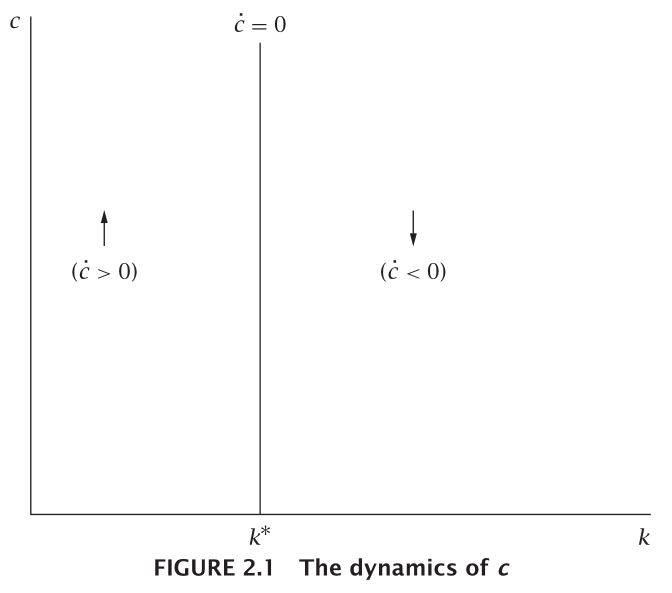
\includegraphics[scale=0.75]{images/cdynamics}
\end{center}

\subsection{Dynamics of $k$}

As in the Solow model, we can also be interested in how $k$ moves over time, especially in the steady state where $\dot k = 0$. From the equation of the dynamics of capital stock per unit of effective labor, we have: $$\dot k = 0 \Leftrightarrow f(k) -(\delta + n + g)k - c^* = 0 \Leftrightarrow c^* = f(k) -(\delta + n + g)k $$ This solution has a trivial value of $c=0$ when $k=0$, but also another solution.

We can see how $c$ moves along the $\dot k = 0$ locus by differentiating with respect to $k$. $$ \frac{\partial c}{\partial k} = f'(k) - (\delta + n + g) $$ Because at $k = 0$ we have $f'(k) = \infty $, we understand that $\frac{\partial c}{\partial k} = \infty$ ; there exists a point $k^G$ where $ f'(k) = \delta + n + g $ leaving $c$ maximized. Finally, at $c=0$ we have two solutions for $k$: $k' = 0$ and $k'' = \frac{f(k'')}{\delta + n + g}$.

As we did for the $\dot c = 0$ locus, we can analyze what happens to the capital stock per unit of effective labor when we deviate from the $\dot k = 0 $ locus. If $c$ is higher than $c^*$ then $\dot k < 0$ for the same level of $k$, and $k$ decreases. If $c < c^*$, then it is the opposite and $k$ increases.

The graph we get is:
\begin{center}
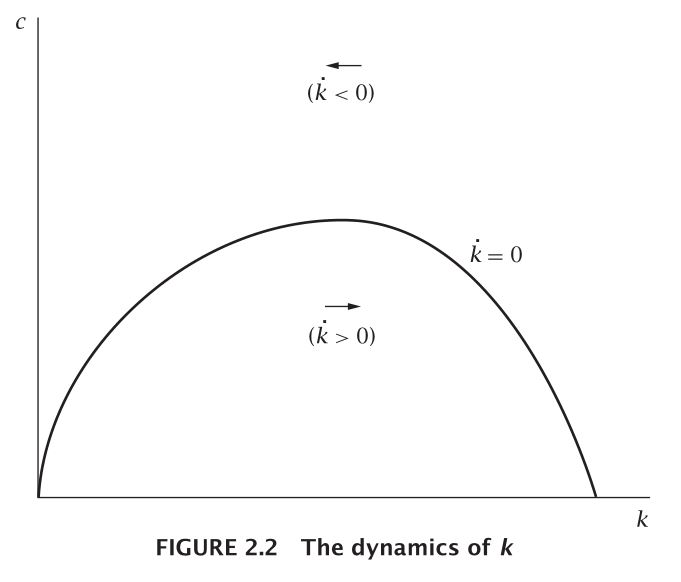
\includegraphics[scale=0.75]{images/kdynamics}
\end{center}

\subsection{Phase diagram}

Putting the two loci together, we get the phase diagram as follows, but we need to understand where the $\dot c =0$ locus stands compared to the $\dot k = 0$ locus. Recall that the $\dot c = 0$ locus is defined by $f'(k^*)  = \delta + \theta g + \rho$ while at the golden-rule level we have $f'(k) = \delta + n + g$. Hence, we need to compare $\theta g + \rho$ to $n + g$. $$\theta g + \rho > n + g \Leftrightarrow \rho - n - (1 - \theta)g > 0 $$ which is true. Therefore the $\dot c = 0 $ locus is at the left of $k^G$, and the phase diagram looks like follows: \begin{center}
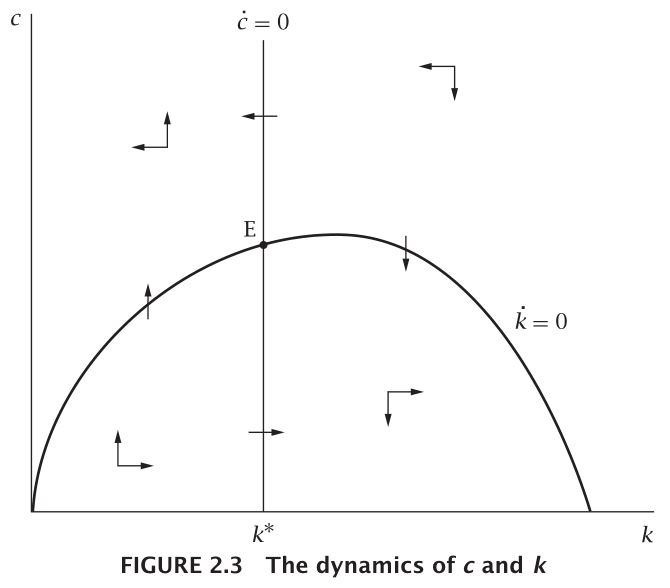
\includegraphics[scale=0.75]{images/Ramseyphase}
\end{center}

The phase diagram shows three crossing points: the origin, point $E$ and $k''$. The origin is not a stable point since increasing the value of either $c$ or $k$ would lead to a better solution. The point at $k''$ is a bit trickier to show its non-stability: we have to use the the transversality condition that states that a consumer cannot hold a positively valued amount of capital at the end of the planning horizon. We are left with the only stable equilibirum $E$.

\subsection{Initial value of $c$}

Now that we know how the economy evolves over time, we can analyze the dynamics of the whole economy from its starting point. The only issue here is that while the initial value of $k$ is known (or assumed) to be $k(0)$, we don't know the initial value of $c$. However this value is extremely important since different values will yield different dynamics as shown below:\begin{center}
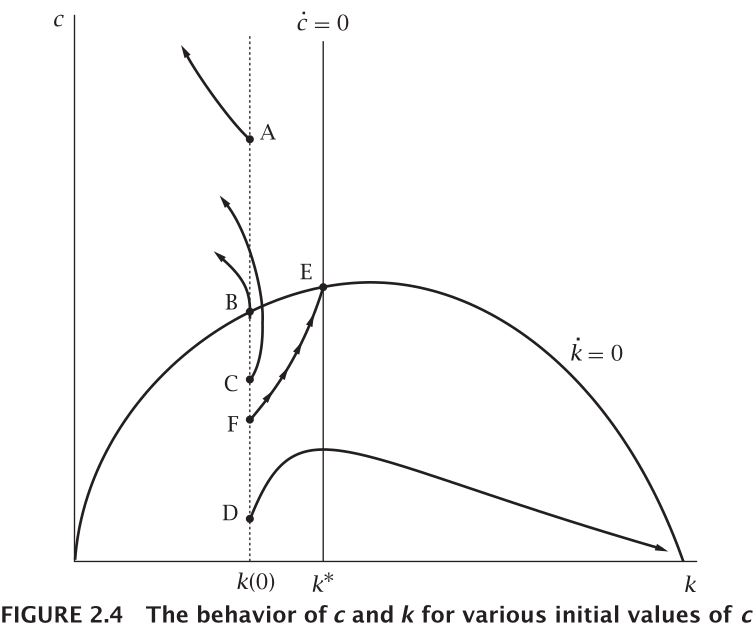
\includegraphics[scale=0.65]{images/Ramseyinitc}
\end{center}
We can clearly see here that only one value of $c(0)$ can lead to the stable equilibrium on $E$. We call the associated trajectory the saddle path of the economy.

\section{Welfare and the BGP}

\subsection{First Welfare Theorem}

The first question that should come to mind to any economist is whether this equilibrium represents a desirable outcome. In this case, the answer is quite simple since every market is perfectly competitive, every agent is rational, there are no externalities of any kind and initial values are consistent with equilibrium. Therefore, the first welfare theorem of general equilibrium must hold: the decentralized equilibrium is equivalent to the social planner's solution. Hence, the equilibrium is Pareto-optimal.

\subsection{Properties of the BGP}

We can show that once equilibrium $E$ is attained, growth of variables are the same as in the Solow model (nothing has changed really once you notice that $\dot c = \dot k = 0$ as in Solow). This is surprising since the savings rate is now endogenous and depends on the state of the economy: the Solow model has the right conclusions it seems. We could also use all implications of the Solow model in regards to cross-country differences and convergence.

\subsection{Social Optimum and Golden-rule}



\section{Impact of a change in the discount rate}

Suppose there is a fall in $\rho$ the discount rate (for consumers). This is analogue to a shock to $s$ in the Solow model. The first difference between shocks in the Ramsey model and in Solow is that because of forward-looking agents, expected shocks have different than unexpected shocks. In fact, it seems obvious that if consumers know that a change will happen, they can prepare before the shock arrives, whereas an unexpected shock will create an immediate reaction only.

\subsection{Unexpected shock}

First of all, we notice that $\rho$ does not enter in the capital motion equation, while it does in the motion equation for consumption. Therefore we can already conclude that the change will affect only the $\dot c = 0$ locus. 

In particular, we know that on that locus, we have: $$f'(k^*) = \delta + \theta g + \rho $$ which implies that the marginal product of capital per unit of effective labor is increasing in $\rho$. This tells us that a fall in the discount rate will yield a decrease of $f'(k^*)$ and hence an increase of $k^*$: the $\dot c = 0$ locus has shifted to the right, we have a new long-run equilibrium, denoted $E'$.\begin{center}
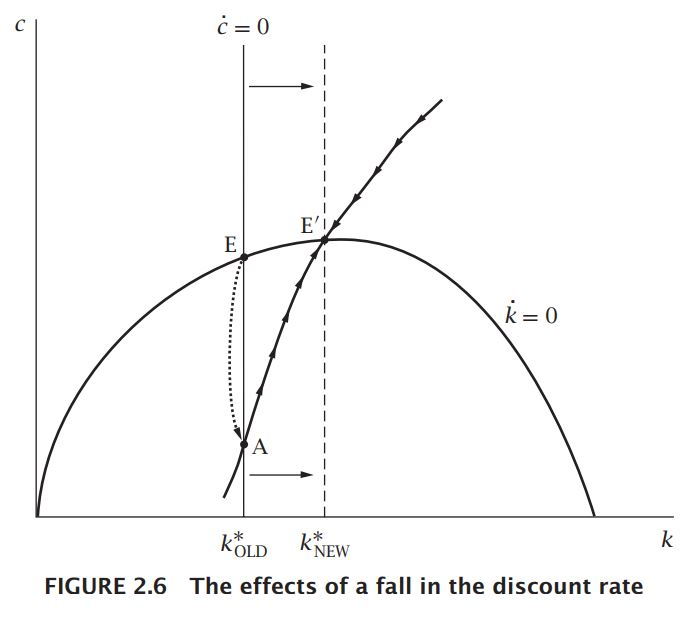
\includegraphics[scale=0.55]{images/Ramseysavingshock}
\end{center}

Now, because our current situation $E$, the level $k$ is too low to maintain a positive growth of $c$. Hence $c$ will jump down. Note that capital does not move because its locus is not affected by the shock at this exact period. Graphically, we can interpret this reaction to the shock as a movement towards the new saddle path. In the period of the shock, consumers are at point $A$ in the above graph, they can move to the new equilibrium point by gradually increasing $c$ and $k$.

\subsection{Expected shock}

If the shock is expected, the effects will change but the new equilibrium will not. If you focus on $E'$ and the new saddle path, you see what consumers expect to be the reality once the shock hits. However, now they have the time to adjust and smooth their transition to the new saddle path. Going back to the phase diagram in figure 2.3, you can see that the only way they can get to the new saddle path is by decreasing consumption and increasing capital (going to the lower right of the diagram). This is not stable and they will drift until they achieve the new saddle path at the same time the shock hits. As a result they have smoothed their transition from $E$ to $E'$.

\subsection{Temporary vs. Permanent shocks}

In the case of expected shocks (or after unexpected shocks), consumers might realize that some shock is only temporary (i.e. it will go back to the previous equilibrium in a finite number of periods). This fact also will change the behavior of consumers, in the same way as an expected shock. Indeed, the end of the shock being foreseeable, it is as if consumers expected a new shock at that period, and thus will act to go smoothly on the new saddle path. If the end of the shock is not known, then it is the same as an unexpected shock.

\section{Impact of Government purchases}

\subsection{The role of government}

\subsubsection{Lump-sum taxes}

In the case of lump-sum taxes, we can say that the government is essentially purchasing output at the place of the consumer and throwing it in the sea. This means that while government expenditures limit the purchase of goods by consumers, it does not affect how they want to allocate consumption over time. Overall, the effect shifts the $\dot k =0$ locus down: consumption jumps down, capital does not move. The government expenditures is perfectly crowding out consumption.

If the shock was temporary, consumers know that at some point they will have to make consumption jump back to the previous equilibrium: this is not desired as it is not smooth enough. What they can do is "take some consumption from the future" in order to smooth. This means dissaving to prevent a decrease in consumption that'd be too big, lowering capital stock, and drifting up and left until the expected saddle path.

\subsubsection{Distortionary taxes}



\chapter{Overlapping Generations Model}

\section{Assumptions}

We now turn to the Diamond overlapping generations model. The central difference between this model and the previous Ramsey model is that people are not infinitely lived. At each period, a fraction of the population will die and a new people will be born. Because of that turnover, we will assume that time is discrete, that is $t=0,1, 2, ...$. Moreover, we will assume that individuals live for only two periods. Even though we will not focus on those assumptions, they turn out to not affect the conclusions of this model.

Assume that $L_t$ individuals are born in period $t$ and that population grows at a rate $n$. Then, $L_t = (1 + n)L_{t-1}$. Moreover, since people only live for two periods, at time $t$ there are $L_{t-1} = L_t/(1+n)$ individuals in their second period of life. An additional assumption on the behavior of these individuals is that, at each period, they provide a fixed amount of labor equal to 1 (regardless of any wage considerations).

Let $C_{1t}$ and $C_{2t}$ denote the consumption of young and old people respectively, at time $t$. Therefore, the utility of an individual born in the period $t$, denoted $U_t$ is defined as a function of both the consumption at time $t$ and at time $t+1$, 
$U_t(C_{1t},C_{2t+1})$

Even though assumptions on firm behavior are still the same, let's review them quickly. We keep our production function with labor-augmenting technology as $Y_t = F[K_t, A_tL_t]$. As before, $F(\cdot)$ displays CRS, satisfies the Inada conditions, and decreasing positive marginal returns. Technology $A_t$ still grows at a rate $g$ so that $A_{t+1} = (1 + g)A_t$. We also still have that $r_t = f'(k_t) - \delta$ and $w_t = f(k_t) - k_tf'(k_t)$. 

Finally, we assume consumers hold capital stock $K_0$ at time $0$. This capital is equally owned by young and old people at the period it's in, it serves as a factor for production. The young individuals divide their labor income $w_tA_t$ between consumption and savings (that goes to capital).

\section{Household behavior}

Let's think of household behavior as a sequential game (and thus solve it by backward induction). In the second period, individuals gain nothing by saving since they will not be alive to see the earnings of those savings. Moreover, they cannot work to earn money. Hence, their consumption in the second period has to come from last period's savings only. Last period's savings is equal to the labor income minus consumption over the first period. We then get: $$C_{2t+1} = (1+r_t)[w_tA_t - C_{1t}] $$ $$\Leftrightarrow \frac{C_{2t+1}}{(1+r_t)} = w_tA_t - C_{1t} $$ This equation gives us the individual's budget constraint as: $$C_{1t} + \frac{C_{2t+1}}{(1+r_t)} = w_tA_t $$ This result is pretty intuitive since it implies that lifetime consumption is equal to initial wealth (here it is $0$) plus the net present value of lifetime consumption.

The individual will choose $C_{1t}, C_{2t+1}$ so that his present utility $U_t$ is maximized subject to this budget constraint. We can solve this maximization problem in two ways: by the perturbation method or by setting up the Lagrangian. For comparison with Fabio's notes we will see the Lagrangian method only. Set up the Lagrangian as: $$\mathcal{L}(C_{1t},C_{2t+1},\lambda) \equiv  U(C_{1t}, C_{2t+1}) + \lambda \left[w_tA_t - C_{1t} - \frac{C_{2t+1}}{(1+r_t)}\right] $$ To simplify calculations, let's assume that utility is a time-separable CRRA function with a discount rate of $1+\rho$. Hence, $$ U(C_{1t}, C_{2t+1}) = \frac{C_{1t}^{1-\theta}}{1-\theta} + \frac{1}{1+\rho}\frac{C_{2t+1}^{1-\theta}}{1-\theta} $$ In the following sections we will continue to assume a CRRA utility function with $\theta > 0$ and $\rho > -1$. Note that the assumption from the Ramsey model that $\rho > n + (1-\theta)g$ is not required anymore. The problem of the consumer becomes: $$\max_{C_{1t},C_{2t+1},\lambda} \frac{C_{1t}^{1-\theta}}{1-\theta} + \frac{1}{1+\rho}\frac{C_{2t+1}^{1-\theta}}{1-\theta} + \lambda \left[w_tA_t - C_{1t} - \frac{C_{2t+1}}{(1+r_t)}\right] $$ which has the following FOCs: $$C_{1t}^{-\theta} = \lambda $$ $$\frac{1}{1+\rho} C_{2t+1}^{-\theta} = \lambda \frac{1}{1+r_t} $$ These two equations can be put together to determine the path of consumption: the Euler equation is back! $$ C_{2t+1} = \left(\frac{1+r_t}{1+\rho}\right)^{\frac{1}{\theta}} C_{1t}$$ We can now replace consumption in the second period inside of the budget constraint: \begin{align*}
C_{1t} + \frac{C_{2t+1}}{(1+r_t)} = w_tA_t & \Leftrightarrow C_{1t} + \frac{1}{(1+r_t)}\left(\frac{1+r_t}{1+\rho}\right)^{\frac{1}{\theta}} C_{1t}  = w_tA_t \\
& \Leftrightarrow C_{1t}\left[ 1 + \frac{(1+r_t)^{\frac{1 - \theta}{\theta}}}{(1+\rho)^{\frac{1}{\theta}}}\right ]  = w_tA_t \\
& \Leftrightarrow C_{1t} = \left( \frac{(1+\rho)^{\frac{1}{\theta}}}{(1+\rho)^{\frac{1}{\theta}} + (1+r_t)^{\frac{1 - \theta}{\theta}}}\right ) w_tA_t
\end{align*} This means that consumption can be written in terms of the income and interest rates, this can be useful if one decides to consider savings as the "opposite" of consumption; in this case, this would give: $$C_{1t} = [1 - s(r_t)] w_tA_t $$ $$ 1 - s(r_t) = \left( \frac{(1+\rho)^{\frac{1}{\theta}}}{(1+\rho)^{\frac{1}{\theta}} + (1+r_t)^{\frac{1 - \theta}{\theta}}}\right ) $$ $$ s(r_t) = 1 - \left( \frac{(1+\rho)^{\frac{1}{\theta}}}{(1+\rho)^{\frac{1}{\theta}} + (1+r_t)^{\frac{1 - \theta}{\theta}}}\right ) $$ $$ s(r_t) = \left( \frac{(1+r_t)^{\frac{1 - \theta}{\theta}}}{(1+\rho)^{\frac{1}{\theta}} + (1+r_t)^{\frac{1 - \theta}{\theta}}}\right)$$ In the particular case of log-utility (i.e. $\theta = 1$), the savings function is a constant: $$s(r_t) = \left( \frac{1}{(1+\rho) + 1}\right) = \frac{1}{2 + \rho}$$ This would a way to micro-found a constant savings rate as in the Solow model for example.

\section{Dynamics of the economy}

\subsection{Equilibrium conditions}

As in the Ramsey model, we can aggregate individuals' behavior to characterize the dynamics of the whole economy. We are particularly interested in how capital stock behaves (as in Solow and Ramsey, we already know what happens to technology and labor). In this model, the capital stock in period $t+1$ is exactly equal to the amount saved by young individuals in period $t$. Recall that it is optimal for the old people to consume all their capital stock in the second period: no capital stock comes from the oldest generation. Thus, $$K_{t+1} = s(r_{t+1})L_tA_tw_t $$ $$\Leftrightarrow k_{t+1} = s(r_{t+1})\frac{L_tA_t}{L_{t+1}A_{t+1}}w_t $$ $$\Leftrightarrow k_{t+1} = \frac{s(r_{t+1})w_t}{(1+n)(1+g)}$$ We can replace the wage and the interest rate by their equilibrium values in the factors' market: $$k_{t+1} = \frac{s(f'(k_{t+1}))[f(k_t) - k_tf'(k_t)]}{(1+n)(1+g)} $$ which is a non-linear first-order difference equation in $k_t$.

\subsection{Evolution of the economy}

\subsubsection{General case}

Solving for the previous general equilibrium condition, we get: $$\frac{\D k_{t+1}}{\D k_t} = \frac{s'(f'(k_{t+1}))f''(k_{t+1})[f(k_t) -k_tf'(k_t)] - s(f'(k_{t+1}))k_tf''(k_t)}{(1+n)(1+g)} $$ which has an unknown shape because of $s'$ which cannot be identified. This raises doubts about the number of potential stable equilibria as well as the very existence of these equilibria. Thus, in the following paragraph, we'll make some assumptions on the behavior so that our model is well behaved.

\subsubsection{Log-utility and Cobb-Douglas economy}

Assuming a log-utility function and a Cobb-Douglas production function, we get: $$ s(r_{t+1}) = \frac{1}{2+\rho} ; f(k_t) = k_t^\alpha ; f'(k_{t}) = \alpha k_t^{\alpha - 1} ; w_t = (1-\alpha)k_t^\alpha $$ Therefore our general equilibrium condition becomes: $$k_{t+1} = \frac{(1-\alpha)}{(1+n)(1+g)(2+\rho)}k_t^\alpha $$ which has a steady-state value (a point for which $k_{t+1} = k_t$). We can compute it as: $k^* = \left(\frac{(1-\alpha)}{(1+n)(1+g)(2+\rho)}\right)^{\frac{1}{1-\alpha}}$ which gives a fairly easy setting to analyze shocks to $n, g, \rho$ or $\alpha$. But as we will see in the next sections, this type of analysis is not what makes the Diamond model most interesting, we will prefer to think about policies in terms of how they interact with the intergenerational side of the model.

\section{Fiscal policies}

\subsection{Lump-sum financed government expenditures}

Denote $G_t$ as the amount of government expenditures per unit of effective labor. Further suppose that this amount if financed via a lump-sum tax on the wage. The wage per unit of effective unit of labor becomes: $w_t = (1-\alpha)k_t^\alpha - G_t $ and thus our previous equilibrium condition becomes: $$k_{t+1} = \frac{(1-\alpha)k_t^\alpha - G_t}{(1+n)(1+g)(2+\rho)} $$

Again, this form gives a fairly easy understanding of what happens following a $G$ shock. We'll have a reduction of $k_{t+1}$ following a positive shock on government expenditures; we also have an increase in $r_t$ (since the marginal product goes up). This conclusion is different from the Ramsey model in which lump-sum financed expenditures left the equilibrium capital stock unaffected after a permanent increase.

\subsection{Bond-financed government expenditures}

This time assume that government expenditures are financed by both lump-sum taxes on wage as well as government bonds. We have that the capital stock and the bonds purchase at time $t$ are equal to the savings ($b_{t+1}$ is the amount of bonds purchased by unit of effective labor at time $t$) such that: $$k_{t+1} + b_{t+1} = \frac{(1-\alpha)k_t^\alpha - T_t}{(1+n)(1+g)(2+\rho)} $$ We also have a government budget constraint (balanced) as: $$\underbrace{T_t + (1+n)(1+g) b_{t+1}}_{\text{Government revenues at time }t} = \underbrace{G_t + [1 + r_t]b_t}_{\text{Government expenditures at time }t} $$ which gives an equation for $T_t$ at the balanced budget condition: $$ T_t = G_t + [1 + f'(k_{t})]b_t - (1+n)(1+g) b_{t+1} $$ which we can use to replace in our general equilibrium condition: $$k_{t+1} = \frac{(1-\alpha)k_t^\alpha - G_t - [1 + f'(k_{t})]b_t + (1+n)(1+g) b_{t+1}}{(1+n)(1+g)(2+\rho)} $$ Hence giving the following result: $$\frac{\D k_{t+1}}{\D b_{t+1}} = \frac{1}{2+\rho} - 1 < 0 $$ implying that a move from taxes to bonds financing will actually reduce $k^*$. The Ricardian equivalence (no crowding-out) does not hold: as the government increases spending from the capital market, the actual level of capital stock decreases.

\section{Social security}

In the setting we just derived, it could be interesting to derive the properties and effects of intergenerational transfers on the evolution of the economy. We'll see two kinds of those transfers, the social security (institutional) and altruism (individual). This section is only on the former.

\subsection{Fully-funded system}

In a fully-funded social security system, young people contribute a certain amount $d_t$ per unit of effective labor. Thus their first period budget constraint is: $$C_{1,t} + s_t + d_t = w_tA_t $$ The government invests the contribution of all young people in the capital stock of the economy, yielding an interest of $r_{t+1}$. Hence, while in their second period the agents receive the interest on their savings and their contribution: $$C_{2,t+1} = (1 + r_{t+1})(s_t + d_t) $$ Hence we can rewrite consumption in the second period as: $$C_{2t+1} = (1 + r_{t+1})(w_tA_t - C_{1t}) $$ $$C_{1t} + \frac{C_{2t+1}}{1 + r_{t+1}} = w_tA_t $$ Consequently, the maximization problem of the young consumer is equivalent to solving the following Lagrangian: $$ \mathcal{L}(C_{1t},C_{2t+1},\lambda) \equiv  U(C_{1t}, C_{2t+1}) + \lambda \left[w_tA_t - C_{1t} - \frac{C_{2t+1}}{(1+r_t)}\right] $$ which must satisfy the following FOCs:\begin{itemize}
\item $C_{1t}^{-\sigma} = \lambda $
\item $\frac{1 + r_t}{1+\rho} C_{2t+1}^{-\sigma} = \lambda $
\end{itemize}
Together these two equations give the same Euler equation as the classical OLG model (without social security), recall: $$ C_{2t+1} = \left(\frac{1+r_t}{1+\rho}\right)^{\frac{1}{\theta}} C_{1t} $$ In the budget constraint: $$w_tA_t = C_{1t} \left( 1 + \frac{1}{1+r_t}\left(\frac{1+r_t}{1+\rho}\right)^{\frac{1}{\theta}}\right) $$ $$\Leftrightarrow w_tA_t = C_{1t} \left( 1 + \frac{(1+r_t)^{\frac{1}{\theta} - 1}}{(1+\rho)^{\frac{1}{\theta}}}\right) $$ $$\Leftrightarrow C_{1t} = w_tA_t \left(\frac{(1+\rho)^{\frac{1}{\theta}}}{(1+\rho)^{\frac{1}{\theta}} + (1+r_t)^{\frac{1-\theta}{\theta}}}\right) $$ Hence, $$s_t + d_t = w_tA_t - C_{1t} $$ $$s_t + d_t = w_tA_t\left(1 - \frac{(1+\rho)^{\frac{1}{\theta}}}{(1+\rho)^{\frac{1}{\theta}} + (1+r_t)^{\frac{1-\theta}{\theta}}}\right) $$

This result seems to be different since $d_t$ is added to the savings, but remember that the potion of social security acquired by the government is also invested in capital. Therefore, the equation of motion of capital is slightly modified to be equal to $k_{t+1} = \frac{s_t + d_t}{(1+n)(1+g)}$. That's why in the end, nothing has changed from the previous model: a social security system where the government saves for you is equivalent of you saving for yourself. This is trivial ex-post because savings by the government exactly offset your own.

\subsection{Pay-as-you-go system}

In a pay-as-you-go system, the mechanism of transfers is slightly different. Instead of investing the participation of young people in capital, the government transfers it to the older generation, thus yielding the rate of $(1+n)$ (remember that population is growing).

Denote the participation at time $t$ by $T_t$. The first period budget constraint is: $$C_{1t} + S_t = A_t w_t - T_t $$ which we can can rewrite to get only the savings: $S_t = A_t w_t - T_t - C_{1t}$. The second-period budget constraint is given by: \begin{align*} C_{2t+1} & = (1+r_{t+1})S_t + (1+n)T_t \\
& = (1+r_{t+1})[A_t w_t - T_t - C_{1t}] + (1+n)T_{t+1}
\end{align*}
which yields the following intertemporal budget constraint of: $$ C_{1t} + \frac{1}{1+r_{t+1}} C_{2t+1} = A_t w_t - T_t + \frac{1 + n}{1+r_{t+1}} T_{t+1} $$

Again, this new form of the budget constraint does not change the Euler equation for consumption which is $C_{2t+1} = \left(\frac{1+r_t}{1+\rho}\right)^{1/\theta} C_{1t}$. In order to simplify calculations, we are going to assume that $\theta = 1$ so that $C_{2t+1} = \frac{1+r_t}{1+\rho} C_{1t}$. Hence we can rewrite the budget constraint to give us the consumption path in terms of income, transfers and participation to the social security: $$C_{1t} \left( \frac{2 + \rho}{1+\rho}\right) = A_t w_t - T_t + \frac{1 + n}{1+r_{t+1}} T_{t+1} $$ $$C_{1t}  = \left( \frac{1 + \rho}{2+\rho}\right)\left[A_t w_t - T_t + \frac{1 + n}{1+r_{t+1}} T_{t+1}\right] $$

Hence, savings in the economy are:\begin{align*}
S_t & = A_t w_t - T_t - C_{1t} \\
& = (A_t w_t - T_t)\left(1 - \frac{1 + \rho}{2+\rho}\right) - \frac{1 + n}{1+r_{t+1}} T_{t+1} \\
& = \frac{(A_t w_t - T_t)}{2+\rho} - \frac{1 + n}{1+r_{t+1}} T_{t+1} 
\end{align*} Now, denote $t_t = T_t/A_t$, we can follow on with the equation for savings: 
\begin{align*}
S_t & = \frac{A_t (w_t - t_t)}{2+\rho} - \frac{(1 + n)A_{t+1}t_{t+1}}{1+r_{t+1}} \\
S_t/A_t & = \frac{w_t - t_t}{2+\rho} - \frac{(1 + n)(1+g)t_{t+1}}{1+r_{t+1}}
\end{align*} 
while the equation of motion for capital is given by: $$K_{t+1} = S_tL_t \Leftrightarrow k_{t+1} = \frac{S_t/A_t}{(1+n)(1+g)} $$ 
$$
k_{t+1} = \frac{w_t - t_t}{(1+n)(1+g)(2+\rho)} - \frac{t_{t+1}}{1+ r_{t+1}}
$$
This new form yields a "shift down" of the usual equation of motion, implying a lower level of $k^*$ on the BGP.


\section{Welfare properties}



\section{Intergenerational altruism}

In this section, we will consider models of over-lapping generations who care about their descendants in a few meaningful manners. In particular, we'll look at how leaving bequests to future generations affect the equilibrium, and how these bequests interact with government expenditures and social security.

\subsection{Simple OLG with Bequests}

Assume that a household born at time $t$ has the following lifetime utility: $$U_t\equiv U(C_{1t}) + \frac{1}{1+\rho} U(C_{2t+1}) + \frac{1}{1+R} U_{t+1} $$ where the first part is the typical lifetime utility and $U_{t+1}$ is the lifetime utility of the next generation, discounted at rate $(1+R)$, a subjective rate. This equation can also be written as a forward sum: $$U_t = \sum_{i=0}^{\infty} \left[ \frac{1}{(1+R)^i} \left( U(C_{1t+i}) + \frac{1}{1+\rho} U(C_{2t+i+1})\right)\right] $$ The budget constraints are slightly modified to introduce the bequest $b_t$ the amount received from the previous generation. Furthermore, we assume no technological progress so that $A_t$ doesn't matter. $$C_{1t} + S_t = w_t + b_t $$ $$C_{2t+1} + (1+n)b_{t+1} = (1+r_{t+1})S_t $$ 

These two constraints will help us rewrite our maximization problem as a discrete-time Bellman equation: $$ U_t = \sum_{i=0}^{\infty} \left[ \frac{1}{(1+R)^i} \left( U(w_{t+i} + b_{t+i} - S_{t+i}) + \frac{U((1+r_{t+1+i})S_{t+i} - (1+n)b_{t+1+i})}{1+\rho} \right)\right] $$ $$ + \lambda_{t+i+1} b_{t+i+1} $$ where the optimizing agent chooses a level of $S_t$ and $b_{t+1}$ to maximize $U_t$. Therefore, the problem must satisfy the following FOCs:\begin{itemize}
\item $ - U'(C_{1t}) + \frac{1+r_{t+1}}{1+\rho} U'(C_{2t+1}) = 0 $
\item $-\frac{1+n}{1+\rho}U'(C_{2t+1}) + \lambda_{t+1} +\frac{1}{1+R} U'(C_{1t+1}) = 0 $
\item and the slackness condition $\lambda_{t+1}b_{t+1} = 0$
\end{itemize}

If $b_{t+1} > 0$, then $\lambda_{t+1} = 0$ and we can rewrite both FOCs as: $$U'(C_{1t}) = \frac{1+r_{t+1}}{1+\rho} U'(C_{2t+1}) $$ $$\frac{1}{1+R} U'(C_{1t+1}) = \frac{1+n}{1+\rho}U'(C_{2t+1}) $$ which imply in turn that in equilibrium: $$ \frac{1+\rho}{1+r_{t+1}} U'(C_{1t}) = \frac{1 + \rho}{(1+R)(1+n)} U'(C_{1t+1}) $$ and at the steady-state, when $C_{1t} = C_{1t+1} = C_1$, we have that: $$ 1 + r = (1 + n)(1 + R) = 1 + \rho$$ if the planner uses the same discount rate as individuals within a generation. Hence, no consumption growth implies $r = \rho$: the same conclusion as the Ramsey model.

\subsection{OLG with bequests and government expenditures}



\subsection{OLG with bequests and social security}




\chapter{Introduction to endogenous growth: One-sector models}

In the three previous types of models (Solow, Ramsey and OLG), we saw that steady-state growth of variables per capita was determined by the rate of technological progress $g$. This is quite an interesting result but it doesn't help us in understanding cross-country differences. In order to understand them, we need models that explain this rate $g$ in an endogenous manner. The simplest way to create endogenous growth in the type of models we know is to allow for increasing returns. This can be done in various ways. This chapter explores some of the ways to model increasing returns to capital and their consequences.

\section{AK model}

The AK model takes the simple production function $y = Ak$ with the underlying assumption that capital is not only restricted to physical capital but can also include human capital, natural resources etc. Hence, it is more plausible to expect increasing returns to scale in the sense that more of this capital can create increasingly more output.

\subsection{Household behavior}

Here we'll use the simple household model derived in the Ramsey model, that is, infinitely-lived optimizing agents with discount rate $\rho$, CRRA utility, etc. Recall, $$U = \int_{t=0}^{\infty} e^{-\rho t} u[C(t)]\frac{L(t)}{H}\D t $$ where $C(t)$ is consumption per capita and $L(t)/H$ is the number of individuals per household. We can write $C(t) = Ac(t)$ where $c(t)$ is the level of consumption per unit of effective labor. Note that in this model $A$ is not a function of time but rather a constant (different than in Ramsey model). Hence, \begin{align*} U & = \int_{t=0}^{\infty} e^{-\rho t} u[Ac(t)]\frac{L(t)}{H}\D t \\
& = \int_{t=0}^{\infty} e^{-\rho t} \frac{[Ac(t)]^{1-\theta}}{1 - \theta}\frac{L(t)}{H}\D t \\
& = \int_{t=0}^{\infty} \frac{A^{1-\theta}L(0)}{H} e^{-\rho t} \frac{c(t)^{1-\theta}}{1 - \theta}e^{nt}\D t \\
& = B\int_{t=0}^{\infty}  e^{-(\rho - n) t} \cdot \frac{c(t)^{1-\theta}}{1 - \theta}\D t 
\end{align*} where we need that $\rho > n$ so that utility doesn't explode over time. The budget constraint is the same as in Ramsey: $$\dot{a} = (r - n)a + w - c$$ We also keep the No-Ponzi-game condition: $$\lim_{t\to\infty}\left\lbrace a(t)e^{-\int_0^t [r(\tau) - n]\D\tau}\right\rbrace \geq 0 $$ which, as in the Ramsey model, implies that the net present value of lifetime assets has to be positive, or in other words, that the debt grows at a rate lower than $r(t) - n$.

Since this problem is essentially the same as in Ramsey, we will not go over the derivation again. The result is the same without $g$, thus: $$\frac{\dot c}{c} = \frac{1}{\theta} [r(t) - \rho] $$

\subsection{Firms behavior}

This section describes the main departure from the Ramsey model. Recall that in this model we have that: $y = f(k) = Ak$ where $A$ is a positive constant. There is no labor, only capital, hence $w = 0$ and $R = f'(k) = A$ implies $r = A - \delta$.

\subsection{Equilibrium}

In equilibrium, again following the Ramsey model, we have: $a = k$ hence: $$\dot k = (r - n)k + w - c$$ where $r = A - \delta$ and $w=0$, yielding: $$\dot k = (A - \delta - n)k - c$$ The second equilibrium condition is: $$\frac{\dot c}{c} = \frac{1}{\theta} [r(t) - \rho]  = \frac{1}{\theta} [A - \delta - \rho]$$ and finally the transversality condition: $$ \lim_{t\to\infty}\left\lbrace k(t)e^{- (A - \delta - n)}\right\rbrace = 0 $$

First of all, notice that consumption growth does not depend on the level of capital this time. We can solve for the path of $c(t)$ as: $$c(t) = c(0) e^{\frac{1}{\theta} [A - \delta - \rho]\cdot t} $$ Thus we will assume that our economy allows for positive growth of consumption over time, meaning that $A > \delta + \rho$. We can replace $c(t)$ in our utility function: \begin{align*}
U & = B \int_{t=0}^{\infty}  e^{-(\rho - n) t} \cdot \frac{c(t)^{1-\theta}}{1 - \theta}\D t \\
& = B \int_{t=0}^{\infty}  e^{-(\rho - n) t} \cdot \frac{[c(0) e^{\frac{1}{\theta} [A - \delta - \rho]\cdot t}]^{1-\theta}}{1 - \theta}\D t \\
& = B\frac{c(0)^{1-\theta}}{1 - \theta} \int_{t=0}^{\infty}  e^{-(\rho - n) t} \cdot [ e^{\frac{1-\theta}{\theta} [A - \delta - \rho]\cdot t}]\D t \\
\end{align*} which requires that $\rho - n - \frac{1-\theta}{\theta} [A - \delta - \rho] > 0$ for utility not to explode.

From the law of motion of capital, we have that $\dot k = 0 \Leftrightarrow c/k = (A - \delta - n)$ a constant. This means that at the steady-state, both variables will have the same growth rate, or formally: $$\frac{\dot k}{k} = \frac{1}{\theta} [A - \delta - \rho] $$ Finally, since $y = Ak$, we also have that $\frac{\dot y}{y} = \frac{\dot k}{k} = \frac{\dot c}{c}$.

\subsection{Phase diagram}

Recall that we have assumed that $A > \rho + \delta$ so consumption will always grow in the steady-state, thus no $\dot c =0$ locus exist, $c$ grows wherever you are on the phase diagram: arrows go up always. For the $\dot k = 0 $ we have seen that it is a line: to the left of the line we have that $c/k$ is too high, $k$ has to decrease, the arrow goes left. The opposite is true when at the right of the line. The phase diagram looks like this:\begin{center}
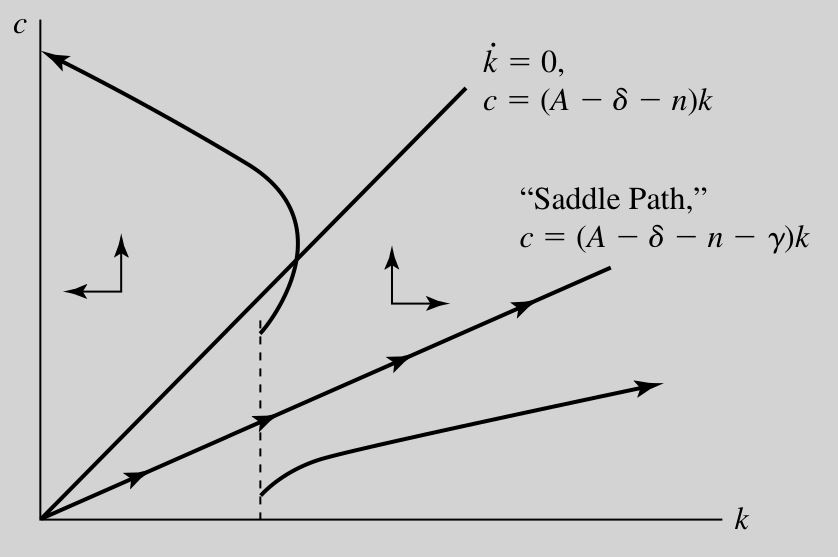
\includegraphics[scale=0.55]{images/akphase}
\end{center}

\subsection{Conclusion}

The main difference between the AK model and the Ramsey model is about long-run growth rates. In the AK model, we see that long-run growth rates are determined by values of $A, \rho$ and $\delta$, while in the Ramsey model only the growth rate of $A$ has an effect on long-run growth.

\section{One-sector model with two types of capital}

In complement to the AK model, where $K$ was believed to represent all forms of capital (encompassing both human and physical capital), this model will keep the one-sector assumption, but will separate both forms of capital.

Let $K$ represent physical capital as usual, while $H$ will be used to denote human capital. The production function is $$Y = F(K, H) $$ where $F(\cdot)$ is a neoclassical production function with CRS, Inada conditions, etc. Using the CRS assumption, we can derive the intensive form of production: $Y = K f(h)$, where $h = H/K$ and $f'(h) > 0$.

As before, we assume that output can be used for consumption or investment (but this time in both forms of capital). Because there are now two types of capital, we'll assume two different rates of depreciation $\delta_H$ and $\delta_K$, as well as two different rental prices $R_H$ and $R_K$. Because of competitive markets we know that firms will equate rental prices to the marginal product of both forms of capital: \begin{align*} 
\frac{\partial F(K,H)}{\partial K} = R_K \Leftrightarrow R_K & = \frac{\partial Kf(h)}{\partial K} = f(h) - K\cdot\frac{H}{K^2}f'(h) = f(h) - h\cdot f'(h) \\\frac{\partial F(K,H)}{\partial H} = R_H \Leftrightarrow R_H & = f'(h)
\end{align*}

Using the fact that both types of capital must be substitutable with each other and with consumption, thus yielding the condition: $r = R_K - \delta_K = R_H - \delta_H$. Hence, $$f(h) - h\cdot f'(h) - \delta_K = f'(h) - \delta_H $$ $$\Leftrightarrow f(h) - (1 + h)f'(h) = \delta_K - \delta_H $$ which is satisfied for a unique value of $h$. Therefore it must be that $f(h)$ is a constant, denote it $A$. We fall back on the AK model since: $$Y = K\cdot f(h) = AK $$

\section{Learning by doing and Knowledge Spillovers}

\subsection{Model}

We have seen in both previous models that a major key in creating endogenous growth is increasing returns to scale. A common way to introduce IRS is to include some kind of positive externalities from production. This section will go over one type of such models, where the externalities come from learning-by-doing assumptions: a firm that increases its physical capital learns how to produce more efficiently.

Consider the production function for one firm: $Y_i = F(K_i, A_iL_i)$ where $L_i$ and $K_i$ are the conventional outputs we are used to, while $A_i$ represents the degree of knowledge available to the firm. We still use our classical assumptions about $F(\cdot)$, but we get rid of the exogenous growth rate of $A$. We will follow two more assumptions that will give to the model its interesting properties.

First, we'll assume learning by doing by linking the "stock" of knowledge $A_i$ to the firm's net investment. Thus, we'll really have that investing in more capital makes you more productive. Note that effectively, the model should be named learning by investing. Second, we'll assume that each firm's knowledge $A_i$ is a public good that any other firm can access. In other words, once new ways of producing more efficiently have been discovered, everyone has access to it. This imply that $\dot A_i$ is somehow linked to the aggregate investment $\dot K$.

Thus, since $A_i$ is proportional to $K$, we can write the production function as: $$Y_i = F(K_i, KL_i)$$ where $K$ and $L_i$ are assumed constant, $K_i$ has decreasing marginal returns, but through investment in $K_i$, a firm can increase $K$ thus making labor more efficient. 

We can write the firm's maximization problem:$$\max_{K_i, L_i} F(K_i, KL_i) - RK_i - WL_i $$ $$\Leftrightarrow\max_{K_i, L_i} L_i[F(k_i, K) - Rk_i - W] $$ which yields the following two FOCs:\begin{itemize}
\item $F'(k_i,K) - R = 0$
\item $F(k_i,K) - k_iF'(k_i,K) - W = 0$
\end{itemize} Moreover, in equilibrium, since all firms are the same, it must be that $k_i = k$ and $K = kL$. Hence, $$F'(k_i, K) = \frac{\partial F(k, kL)}{\partial K_i} =  \frac{\partial k_i f(L)}{\partial K_i} = f(L) - Lf'(L)$$

\subsection{Equilibrium}

We now have that $r = f(L) - Lf'(L) - \delta$ which we can use for the consumption path locus: $$\frac{\dot c}{c} = \frac{1}{\theta} [ f(L) - Lf'(L) - \delta - \rho ] $$ This equation is similar to the one derived in the AK model, implying that here as well, consumption growth is constant as long as $L$ is constant. In the capital growth equation we have: $$\dot k = f(L)k - c - \delta k $$ Therefore, in the same way as in the AK model, we have growth dynamics that are dependent on $\dot c/c$ and yield endogenous growth of the economy.

\subsection{Pareto nonoptimality}

This model brings a new topic that is interesting enough to be described here: Pareto optimality. So long we have talked about this only in OLG models where some distortions were introduced in the models, here, we have in fact a distortion: the knowledge spillover. In fact, as in most cases with externalities, firms do not internalize these externalities in their behaviour (they take $K$ as given), yielding a sup-optimal equilibrium. To see that, let's analyze the optimal allocation by studying the maximization problem of a benevolent social planner.

The objective of the social planner is to maximize utility of consumption while respecting the economy's budget constraint. This is equivalent to maximizing the following: $$\max_{c, k} \int_0^\infty e^{-\rho t} \frac{c(t)^{1-\theta}}{1 - \theta}\D t \text{ s.t. } \dot k(t) = f(L)\cdot k(t) - c(t) - \delta k(t) $$ we get the following Hamiltonian: $$H\equiv e^{-\rho t} \frac{c(t)^{1-\theta}}{1 - \theta} + \lambda(t) \cdot [f(L)\cdot k(t) - c(t) - \delta k(t)] $$ which gives the following conditions:\begin{itemize}
\item $ e^{-\rho t} c(t)^{-\theta} = \lambda(t) \Leftrightarrow (-\rho - \theta \dot c(t)/c(t)) = \dot \lambda (t)/ \lambda(t)$
\item  $\dot \lambda(t) = - \lambda(t)[f(L) - \delta] \Leftrightarrow  \dot c(t)/c(t) = (1/\theta)\cdot [f(L) - \delta -\rho] $
\end{itemize} where you can clearly see already that the growth rate of consumption is greater than in the individual maximization case. This means that our previous model is exactly as we expected, non-optimal in the Pareto sense.

In order to make it more optimal, we should regulate to make firms internalize the gains of knowledge spillovers (or complete the wedge between individual marginal product and social marginal product). This can be achieved by lump-sum credit on investment to incentivize more investment.

\subsection{Scale effects}

Another interesting implication of the learning-by-doing model is the apparition of scale effects in our model. Indeed, since consumption growth depends directly on the level of labor (or equivalently population) it would mean that a bigger population would yield a higher growth.

Discussion?

\section{Public goods model}

Following the previous models, we show in this section that including public goods can help in creating increasing returns to scale.

\subsection{Basic model}

Let government expenditures $G$ enter in the firms production function as a public good (all firms experience the same level of $G$). For each firm, the production function is thus: $$ Y_i = AL_i^{1-\alpha}K_i^{\alpha}\cdot G^{1-\alpha} $$ We still have a neoclassical function in the sense that there are constant returns to scale in private inputs. The main difference is that a growing $G$ alongside an input will generate constant returns ($K$) or even increasing returns ($L$ if $\alpha < 0.5$). These types of returns will allow endogenous growth.

In order to finance its expenditures, the government taxes households via a lump-sum tax (no distortion). This has no effect on the optimal behavior of the household, and thus leaves the Ramsey result we've been using in this chapter unchanged.

For the firms, we have that the rental rate of capital is given by: $$R = \alpha A L_i^{1 - \alpha} K_i^{\alpha - 1} \cdot G^{1-\alpha} = \alpha A  k_i^{-(1 - \alpha)} \cdot G^{1-\alpha} $$ This implies that all firms will choose the same level $k_i$ in equilibrium (perfect competition and price-taking assumptions). We can aggregate the production function to: $Y = ALk^\alpha G^{1-\alpha} $. This can be rewritten in the following form: $$ G = \left( ALk^{\alpha}\cdot (G/Y) \right)^{1/\alpha} $$ which emphasize the role of the public spending share in GDP ($G/Y$). Suppose the government chooses its spending level to keep the public spending share constant. Replacing in the rental rate for capital we get: $$R = \alpha A  k_i^{-(1 - \alpha)} \cdot \left( ALk^{\alpha}\cdot(G/Y)\right)^{(1-\alpha)/\alpha} = \alpha A^{1/\alpha}L^{(1-\alpha)/\alpha} \cdot (G/Y)^{(1-\alpha)/\alpha} $$ 
You can clearly see that, if labor and the public spending share are constant, our model has a steady-state. This gives the same kind of results as in the AK model, no transitional dynamics (any shift in parameters will result in a jump to the new growth rate). Recall that you need to plug the rental rate in consumption growth (the $\dot c/c$ result) to see that: this should be automatic by now. The model also predicts scale effects ($L$ shifts consumption growth).

\subsubsection{Distortionary taxes}



\subsubsection{Optimal public spending}

Return to the model with lump-sum taxes, one good question to ask ourselves at this moment is what would be the best public spending share. In order to compute it, we need to find the share such that an additional dollar of public spending yields at least more than one dollar in output or more formally: $\partial Y/\partial G = 1$. $$\frac{\partial Y}{\partial G} = 1 \Leftrightarrow (1 - \alpha) \frac{Y}{G} = 1 \Leftrightarrow (G/Y) = 1 - \alpha $$ This particular share would be the one used by a social planner: any different level would be non-optimal in the Pareto sense. We can show it by writing the Hamiltonian. Recall that in the social planner's problem, we can write $(R - \delta)k + w = (Y/L) - \delta k$ in the constraint since market clearing is internalized (here, you do not divide variables by A since it is a constant). Hence, the resource constraint becomes: $\dot k = (Y/L) - \delta k - c - G/L$ in this problem. \begin{align*}
 H & \equiv e^{-\rho t} \frac{c^{1-\theta}}{1-\theta} + \lambda\left[ Ak^\alpha G^{1-\alpha} - \delta k - c - G/L\right]
\end{align*} yielding the following conditions (given the optimal C and G, find lambda and k):\begin{itemize}
\item C: $e^{-\rho t} c^{-\theta} = \lambda $
\item G: \begin{align*}
\lambda \left( (1-\alpha) Ak^\alpha G^{-\alpha} - L^{-1} \right) = 0 & \Leftrightarrow (1-\alpha) A k^\alpha \left( ALk^{\alpha}\cdot (G/Y) \right)^{-1} = L^{-1} \\
& \Leftrightarrow (1-\alpha) = (G/Y)
\end{align*}
\item Lambda: $-\dot\lambda = \alpha A^{1/\alpha}L^{(1-\alpha)/\alpha} \cdot \left(\frac{G}{Y}\right)^{(1-\alpha)/\alpha} - \delta $
\end{itemize}
Mixing the equations together as in the Ramsey model yields: $$(\dot c/c)^* = \frac{1}{\theta}\left[ A^{1/\alpha}L^{(1-\alpha)/\alpha} \cdot \left(1-\alpha\right)^{(1-\alpha)/\alpha} - \delta - \rho \right] $$

\subsection{Congestion model}

Following the previous model, a natural expansion would be to look at the case where government spending has some kind of a limit. In fact, in the previous model, we could expand $G$ by how much we wanted until $\partial Y/\partial G$ was lower than one. In the following model, we assume that there is "congestion" in public spending. This means that for a given level of $G$, an increase in output $Y$ will create congestion: less usage of the same public goods. We model it as the following individual production function: $$ Y_i = A K_i\cdot f\left(\frac{G}{Y}\right) $$ where the function $f(\cdot)$ is a concave function.

Again, adding this type of government spending does not affect consumer behavior: we can use the Ramsey result.

The rental rate for capital is given by: $$ R = A \cdot f\left(\frac{G}{Y}\right) $$ which is independent of individual firms decisions, meaning that all firms use the same level $K_i = K$. The growth rate of $c$ is given by: $$\dot c/c = 1/\theta \left[ A \cdot f\left(\frac{G}{Y}\right) - \delta - \rho \right] $$ The main difference here is the absence of scale effects in this particular model.

\subsubsection{Pareto optimality}

In this model too we can compare the previous solution to the solution of the social planner: $$H \equiv e^{-\rho t} \frac{c^{1-\theta}}{1-\theta} + \lambda\left[\left(A \cdot f\left(G/Y\right) - \delta\right)k - c - G/L\right] $$

\section{Kremer model}

The last model of this chapter is the one Kremer devised 

Assume a simple production function using a fixed amount of land $T$, and the usual effective labor $AL$ to produce output. $$ Y = T^\alpha (AL)^{1-\alpha} $$ Moreover, assume that knowledge growth (or technology) is proportional to both knowledge itself and population such that: $$ \dot A = B\cdot L \cdot A^{\theta} $$ Finally, suppose that output per capita is constant, equal to a "subsistence level" (Malthusian assumption): $$ Y/L = \bar y $$

To solve this model, we need only labor growth (we already know technology growth and land growth). From the previous three assumptions, we can solve for labor: $$ \frac{T^\alpha (AL)^{1-\alpha}}{L} = \bar y \Leftrightarrow L^\alpha = \frac{T^\alpha A^{1-\alpha}}{\bar y}  \Leftrightarrow L = T A^{(1-\alpha)/\alpha}\frac{1}{\bar y} $$ This allows for a simple expression for labor growth: $$\dot L/L = \frac{1-\alpha}{\alpha} \left(\dot A/A\right) = \frac{1-\alpha}{\alpha} \left( B L \cdot A^{\theta - 1} \right) $$ This equation implies that population growth is proportional to the population level and to technology. We get a circle of feedback effects: more population means more population and more technology, which in turn imply more population and more technology. This is the kind of result that we would expect from an AK model (endogenous growth) with characteristics form the learning by doing or by public spending (scale effects).

\chapter{Two-sectors model}

We have seen that the inclusion of two different types of capital, namely physical ($K$) and human ($H$) capital can help to remove diminishing returns and provide an explanation for endogenous growth models. In the previous chapter, we included both types but only one type of investment: we ended up on the AK model. In this chapter, we'll make the distinction increasingly clearer by first differentiating both types of investments, then allowing for different production functions and finally consider the setting where the two forms of capital are differently intensive in labor.

\section{One-sector model with physical and human capital}

\subsection{Assumptions}

We start with a typical Cobb-Douglas production function with CRS in both forms of capital and which satisfies Inada conditions. Let $Y = AK^\alpha H^{1 - \alpha}$ where $H$ is human capital, determined by $L$ the number of workers and $h$ the human capital of a worker. Since $H = Lh$, we have that hours worked and human capital are exactly substitutable at all times. For convenience, we'll further assume that $L$ is fixed, leaving only $h$ to move $H$. We'll also assume that $A$, technology in this model, is fixed.

Both types of investment have the same rate of depreciation by assumption, so that: $$\dot K = I_K - \delta K \text{ and } \dot H = I_H - \delta H $$ while the economy's resource constraint is $Y = C + I_K + I_H $.

\subsection{Equilibrium}

As usual, we solve for the economy's dynamics in equilibrium by solving the consumer's problem subject to the economy's resource constraint as well as the dynamics constraint: $$\max_{c, k} \int_0^\infty e^{-\rho t} \frac{c^{1-\theta}}{1 - \theta}\D t \text{ s.t. } \begin{cases} \dot K & = I_K - \delta K \\
\dot H & = I_H - \delta H \\
Y & = C + I_K + I_H
\end{cases} $$ which gives the following Hamiltonian equation: $$ H\equiv e^{-\rho t} \frac{c^{1-\theta}}{1 - \theta} + \mu [I_K - \delta K] + \nu [I_H - \delta H] + \omega [AK^\alpha H^{1 - \alpha} - C - I_K - I_H ] $$ which gives the following conditions:\begin{itemize}
\item $e^{-\rho t} c^{-\theta} = \omega \Leftrightarrow (-\rho - \theta \dot c/c) = \dot \omega / \omega $
\item $\mu = \omega$
\item $\nu = \omega$
\item $\dot\mu = [\mu\delta - \omega A\alpha K^{\alpha -1 }H^{1 - \alpha}] \Leftrightarrow (\dot\mu /\mu)= [\delta - A\alpha K^{\alpha -1 }H^{1 - \alpha}]$
\item $\dot\nu = [\nu\delta - \omega A(1-\alpha) K^{\alpha}H^{- \alpha}] \Leftrightarrow (\dot\nu /\nu)= [\delta - A(1-\alpha) K^{\alpha}H^{- \alpha}]$
\end{itemize} which finally yields: $$\frac{\dot c}{c} = \frac{1}{\theta} [A\alpha(K/H)^{-(1-\alpha)} - \delta - \rho] = \frac{1}{\theta} [A(1-\alpha)(K/H)^{\alpha} - \delta - \rho]$$ These last two equations put together can give another condition to our model: $(K/H) = \alpha/(1-\alpha)$. This means that the ratio of physical capital over human capital is constant! Therefore the rate of return of either has to be constant as well: $$r^* = A\alpha^\alpha\cdot(1-\alpha)^{1-\alpha} - \delta $$ and moreover, the consumption growth locus is constant as well:$$ \frac{\dot c}{c} = \frac{1}{\theta} [A\alpha^\alpha\cdot(1-\alpha)^{1-\alpha} - \delta - \rho]$$ We can clearly see a link with the AK model presented in the previous chapter, and in fact, by CRS, we can find: $$Y = AK\left(\frac{1-\alpha}{\alpha}\right)^{1-\alpha} $$ which is a form of an AK model.

\section{Two-sectors model}

\subsection{Basic Model}

\subsubsection{Assumptions}

We have assumed, thus far, that physical goods and education are generated by the same production function. However, it might be more realistic to depend more on educated people to produce education than physical goods, and vice versa. Therefore, we'll modify our model to allow for one production function for each type of good. As before, the production of consumption goods is $$ Y = A(vK)^{\alpha}\cdot(uH)^{1-\alpha} = C + \dot K + \delta K $$ where $v,u\in (0,1)$ are the shares of the total stock of $K$ and $H$ respectively, that are used in the production of goods. We also have now that the production of human capital is: $$I_H = B\cdot[(1-v)K]^\eta \cdot [(1-u)H]^{1-\eta} = \dot H + \delta H$$ Note that if $\eta = \alpha$, then both production functions are equivalent and we are back to the one-sector model of last section. However, accounting for the fact that the education sector is more intensive on capital ($\eta < \alpha$), we get two different production functions.

\subsubsection{Equilibrium}

We have the following Hamiltonian: $$ H\equiv e^{-\rho t} u(C) + \nu [ A\cdot (vK)^\alpha \cdot (uH)^{1-\alpha} - \delta K - C] + \mu [B\cdot[(1-v)K]^\eta \cdot [(1-u)H]^{1-\eta}] $$ satisfying the following conditions:\begin{itemize}
\item $e^{-\rho t} u'(C) = \nu$
\item $\nu A K^{\alpha}H^{1-\alpha} (u/v)^{1 - \alpha} = \mu B K^\eta H^{1-\eta} [(1-u)/(1-v)]^{1 - \eta} $
\item $\nu A K^{\alpha}H^{1-\alpha} (u/v)^{- \alpha} = \mu B K^\eta H^{1-\eta} [(1-u)/(1-v)]^{- \eta} $
\item[ ] which gives $ u/v = (1-u)/(1-v) \Leftrightarrow [u/(1-u)] = [v/(1-v)] $
\item 
\end{itemize}

\subsection{Uzawa-Lucas Model}



\section{Summary}



\chapter{Endogeneizing Technological Change}

We have seen that allowing our models to have endogenous growth is possible when you go away from diminishing returns. This view implies that growth can arise even in the absence of  technological growth. However, this view also implies that accumulation of capital (in its broader form) never stops, even though it would seem more probable that at some point the rate of return has to decline. Then, we'd need to go back to technological progress as a source of growth. In both the Solow and Ramsey models, we explored the dynamics of an economy with an exogenous technological progress; in this chapter, we will cover a few models that try to provide an endogenous explanation to this growth.

\section{Expanding variety of products models}

This model is telling the story in which technological growth comes from the continuous increase in the number of products available in the economy. In other words, technology is increasing with the complexity of inventions made. In order to set up a model like this one, we need three agents: the firms, the consumers (as usual) and R\& D firms. Firms will use a combination of labor and intermediate inputs (no capital) to produce a unique output. These intermediate inputs are created by the R\& D firms. Finally, consumers play their typical role (as in Ramsey). To solve the model, we'll use a type of backwards induction, looking at behavior from firms, then R\& D companies (consumers are unchanged so not really important).

\subsection{Producers of final output}

As we said earlier, the producers of final output have access to a production technology that combines both labor and intermediate inputs of different types, denoted $X_j$ where $j\in 1, 2, ..., N$ with $N$ being the number of intermediate goods available (variety of products). Therefore, each firm can produce: $$ Y_i = AL_i^{1-\alpha}\sum_{j=1}^{N}(X_{ij})^\alpha $$ This form has quite a few interesting properties. First, notice that the Cobb-Douglas form specifies diminishing marginal returns for any input ($L_i$ or $X_ij$) and constant returns to scale in both inputs. Moreover, the additive separability of the intermediate inputs implies that their respective marginal return is independent of the others. Third, for each intermediate product, its marginal productivity is infinite when not used: all of them are used. Finally, if we assume that a firm uses the same level of each input (which should hold in equilibrium  as they are not differentiated in their participation to output), then $X_{ij} = X_i$ and $\sum_{j=1}^{N} X_{ij} = NX_i$ and we get: $$Y_i = AL_i^{1 -\alpha} NX_i^\alpha = AN^{1 -\alpha}L_i^{1 -\alpha} (NX_i)^\alpha$$ This new form show that $N$ actually increases output.

The output $Y$ can be used for consumption or the production of intermediate goods. Note that it would be possible to introduce capital in this model by modeling $X$ as service flows for a given physical capital rented by intermediate firms. This analysis yields the same result so we'll keep with the simpler model. Final output firms maximize: $$\max_{L_i, X_{ij}} AL_i^{1-\alpha}\sum_{j=1}^{N}(X_{ij})^\alpha - wL_i - \sum_{j=1}^{N}P_jX_{ij} $$ which satifies the following FOCs:\begin{itemize}
\item $(1-\alpha) AL_i^{-\alpha}\sum_{j=1}^{N}(X_{ij})^\alpha - w = 0 \Leftrightarrow w = (1-\alpha)(Y_i/L_i) $
\item $\alpha A L_i^{1-\alpha} X_{ij}^{\alpha - 1} - P_j = 0 \Leftrightarrow X_{ij} = L_i \left[\frac{\alpha A}{P_j}\right]^{\frac{1}{1-\alpha}}\quad \forall j\in 1, ..., N $
\end{itemize} which can be interpreted as input conditional demands. Now we can look at what happens to the providers of these inputs, namely research firms and consumers

\subsection{Research Firms}

At a point in time, the technology exists to produce $N$ varieties of intermediate goods. In order to increase this variety, we require a technological advance (an invention of a new product) that will be done by a research firm. These firms are assumed to take their decisions based on a two-step game, first they decide if they will or won't invent the new product, then they get the profits of inventing the new product or not. Thus, we'll solve their decision as a sequential game: by backwards induction.

\subsubsection{Step 2: Profit if a new product is developed}

In order to motivate research, successful innovators need to be compensated. We'll assume that they get a monopoly rent on their product (they are the only one allowed to produce a particular good that they invented). Therefore, their lifetime profit is the net present value of their profits at each point in time, starting from the period in which they invent the profit $t$ to infinity. For a product $X_j$, this is written as: $$V(t) = \int_t^\infty \pi_j(v)\cdot e^{-\bar r(t, v)\cdot(v-t)} \D v $$ where $\pi_j(v)$ is the profit flow at each point in time $v$ and $\bar r(t, v)$ is the average discounting rate effective from time $t$ to $v$. If this rate is constant, then $\bar r(t, v) = r$.

Their profit flow comes from the revenues from the sale of the intermediate goods minus the costs: $\pi_j(v) = [P_j(v) - 1]X_j$ where $X_j = \sum_{i} X_{ij}(v) = \sum_{i} L_i \left[\frac{\alpha A}{P_j(v)}\right]^{\frac{1}{1-\alpha}} = \left[\frac{\alpha A}{P_j(v)}\right]^{\frac{1}{1-\alpha}} \cdot \sum_{i} L_i = \left[\frac{\alpha A}{P_j(v)}\right]^{\frac{1}{1-\alpha}} \cdot L$. Thus, when they choose the price to maximize that profit, it must satisfy: $$\left[\frac{\alpha A}{P_j(v)}\right]^{\frac{1}{1-\alpha}} \cdot L - \frac{1}{1-\alpha}[P_j(v) - 1]\cdot \left[\frac{\alpha A}{P_j(v)}\right]^{\frac{1}{1-\alpha}} \cdot L\cdot P_j(v)^{-1} = 0 $$ $$ \frac{[P_j(v) - 1]}{P_j(v)} = 1-\alpha $$ $$P_j(v) = \frac{1}{\alpha} > 1 $$ At this price point, the demand for the product $X_j$ is $$ X_j = (\alpha^2 A)^{\frac{1}{1-\alpha}}\cdot L $$ 

Aside that, we can also retrieve aggregate demand for intermediate goods and aggregate output as: $$X = NX_j = (\alpha^2 A)^{\frac{1}{1-\alpha}}\cdot LN $$ $$ Y = A L^{1-\alpha} [(\alpha^2 A)^{\frac{1}{1-\alpha}}\cdot LN]^{\alpha} \cdot N^{1-\alpha} = A^{\frac{1}{1-\alpha}} \alpha^{\frac{2\alpha}{1-\alpha}} LN $$ which also gives that $X = \alpha^2 Y$.

Back to the research firms, we have their profit flow is given by: $$\pi_j(v) = \pi = \left(\frac{1-\alpha}{\alpha}\right)\cdot(\alpha^2 A)^{\frac{1}{1-\alpha}}\cdot L $$ 

\subsubsection{Step 1: Will they make the new product?}

We now know the amount of profit realized once a good has been done. Now, in order for this product to be actually invented, we need that this profit outweighs R\& D costs of making it. In this model, we'll make the very simplifying assumption that these costs amount to $\eta$ units of the final good. Therefore, any R\& D firm will devote resources to making a new product if and only if $V(t)>\eta $.

\subsubsection{Free-entry condition}

The free-entry assumption is crucial in solving this model. In fact, letting firms enter freely imply that in the long run, no excessive profits will be made so that $V(t) = \eta$. We call this equation the free-entry condition. Differentiating this condition with respect to time yields that the interest rate is constant over time, equal to: $$r = (L/\eta)\cdot A^{\frac{1}{1-\alpha}} \cdot \left(\frac{1-\alpha}{\alpha}\right)\cdot\alpha^{\frac{2}{1-\alpha}} $$

\subsection{Households}

Finally, we need to model household behavior to close the model. Fortunately, this is quite easy since we did not assume any new elements from Ramsey, therefore: $$\frac{\dot c}{c} = \frac{1}{\theta} [ r - \rho] $$

\subsection{Equilibrium}

Now, in a closed economy, it must be that the total value of firms is equal to the total value of assets: $\text{assets} = \eta\cdot N$. Moreover, since we assumed that $\eta$ is constant, we also have that: $\dot{\text{assets}} = \eta \dot N $. On the labor market, we have that $w = (1-\alpha)(Y/L)$ while on the assets market we get $r = \frac{1}{\eta} (1-\alpha)\alpha (Y/N) $. Hence, total income is given by $$wL + r\cdot(\text{assets}) = (1-\alpha)Y + (1-\alpha)\alpha Y = Y(1-\alpha)(1+\alpha) = Y(1 - \alpha^2) $$ Moreover, we've previously derived that: $X = \alpha^2 Y$. These two equations  will help us derive the budget equation for the economy. At the consumer's level, total income minus consumption represents the amount that is used to buy assets: $$\dot{\text{assets}} = wL + r\cdot(\text{assets}) - C $$ $$ \eta \dot N = Y(1 - \alpha^2) - C = Y - C - X $$ This equation states the dynamics of the expanding variety of products $N$ (as if it was capital in Ramsey). It must be used with the dynamics of consumption, given by: $$ \frac{1}{\theta} \left[ (L/\eta)\cdot A^{\frac{1}{1-\alpha}} \cdot \left(\frac{1-\alpha}{\alpha}\right)\cdot\alpha^{\frac{2}{1-\alpha}} - \rho\right] $$

Because every variable depends on $C$, we have that the previous equation pins down the dynamics of the entire economy.

\subsection{Determinants of the growth rate}

The determinants of the growth rate are therefore the parameters present in the dynamic equation for consumption, namely, $L, \eta, A, \alpha$ and $\rho$.

\subsection{Pareto Optimality}

Again, since this model is showing some signs of market power, we might get a different optimum in the individual optimization case and in the social planning case. Specifically, the social planner can internalize the welfare losses of having a monopoly in the R\& D sector. Therefore, growth in the individual problem is lower than the social planner's solution. There are a few potential solutions to this issue:\begin{itemize}
\item Subsidies on the price of intermediate goods
\item Subsidies to the final product
\item Subsidies to research
\end{itemize}

\section{Quality Ladder models}



\section{Models with technology diffusion}

\chapter{Explaining cross-country income differences}

\section{Extended Solow model}

This model follows from Mankiw, Romer and Weil and presents a view of the Solow model accounting not only for physical capital and labor but also human capital.

\subsection{Model}

Consider the following production function: $$Y = K^\alpha H^\beta (AL)^{1-\alpha-\beta} $$ where $\alpha, \beta > 0$ and $\alpha + \beta < 1$. As we see, there are now two types of capital in which households can invest. MRW make the assumption that both have the same depreciation rate but different savings rate $s_K$ and $s_H$ (exogenously set, as in the Solow model). The laws of motion for this model are therefore: $$\dot K = s_K\cdot Y - \delta K\quad \text{ and } \quad \dot H = s_H\cdot Y - \delta H $$ We can write the model in terms of variables per unit of effective labor (dividing by $AL$). This yields: $$\frac{Y}{AL} = \left(\frac{K}{AL}\right)^\alpha\cdot \left(\frac{H}{AL}\right)^\beta \cdot \frac{AL}{AL} \Leftrightarrow y = k^\alpha h^\beta $$ The same goes for the laws of motion for both types of capital: $$\frac{\partial \frac{K}{AL}}{\partial t} = \frac{\dot K (AL) - K(\dot A L + A\dot L)}{(AL)^2} = \frac{\dot K}{AL} - k\left(\frac{\dot A}{A} + \frac{\dot L}{L}\right) = s_K y - \delta k - (n + g) k $$ which divided by $k$ gives: $\dot k/k = s_K(k^{\alpha - 1}h^\beta) - (\delta + n + g) $. In the same way, we can find the law of motion for human capital per unit of effective labor as: $\dot h/h = s_H(k^{\alpha}h^{\beta- 1}) - (\delta + n + g) $.

Recall that the consumption side is irrelevant here since the savings rate is exogenously defined. Our model is now set, we can go on to study the steady-state.

\subsection{Steady-state}

In the steady-state, both laws of motion derived should equal to zero. Let's find out their expression in that case.

\subsubsection{Physical capital steady-state}

\begin{align*}
\dot k/k = 0 \Leftrightarrow s_K(k^{\alpha - 1}h^\beta) - (\delta + n + g) = 0 & \Leftrightarrow s_K(k^{\alpha - 1}h^\beta) = \delta + n + g \\ & \Leftrightarrow \left(\frac{s_K}{\delta + n + g}\right)\cdot h^\beta = k^{1-\alpha} \\
& \Leftrightarrow  k = \left(\frac{s_K}{\delta + n + g}\right)^{\frac{1}{1-\alpha}}\cdot h^{\frac{\beta}{1-\alpha}}
\end{align*} This is a concave function of $h$ since $\beta < 1 -\alpha$. We can draw it in the $(k, h)$ space as the $\dot k/k = 0$ locus.

\subsubsection{Human capital steady-state}

\begin{align*}
\dot h/h = 0 \Leftrightarrow s_H(k^\alpha h^{\beta - 1}) - (\delta + n + g) = 0 & \Leftrightarrow s_H(k^{\alpha}h^{\beta - 1}) = \delta + n + g \\ & \Leftrightarrow \left(\frac{s_H}{\delta + n + g}\right)^{-1}\cdot h^{1 - \beta} = k^{\alpha} \\
& \Leftrightarrow  k = \left(\frac{s_H}{\delta + n + g}\right)^{-\frac{1}{\alpha}}\cdot h^{\frac{1 -\beta}{\alpha}}
\end{align*} This is a convex function of $h$ since $\beta < 1 -\alpha$. We can draw it in the $(k, h)$ space as the $\dot h/h = 0$ locus.

\subsubsection{General steady-state}

Since one locus has a decreasing derivative and the other has an increasing one, both will have a meeting point. The objective is to find the values $(k^*, h^*)$ such that $\dot k/k = \dot h/h = 0$.

\section{Empirical evaluation}



\section{Social infrastructure}



\section{Beyond social infrastructure}



\chapter{Stochastic Dynamic Programming}

\section{Investment with adjustment costs}

Consider a firm which is assumed to maximize its market value (the sum of its dividends). In order to do that, it must invest in capital (which will guarantee higher profits in the future) but also give out dividends (to ensure its market value). We take its problem as maximizing $$M \equiv \Et{\sum_{s=0}^{\infty} \beta^s D_{t+s}} $$

Its investment is the value of capital that is added at each period plus the cost of maintaining its current capital: $I_t = K_{t+1} - K_t + \delta K_t$. Moreover, the dividend it can give out must be equal to the firm's profit minus its investment and adjustment costs necessary when new capital is introduced (this is a new assumption). Therefore we can write: $$D_t = \pi(\zeta_t)\cdot K_t - \frac{b}{2}\left(\frac{I_t}{K_t}\right)^2K_t - P_t^II_t $$ where $\pi(\zeta_t)$ is the expected profit per unit of capital engaged and $P_t^I$ is the price of investing money (borrowing costs). The Bellman equation for that problem is: $$V_t(K_t,\zeta_t) = \max_{I_t} D_t + \beta\Et{V_{t+1}(K_{t+1}, \zeta_{t+1})}  $$ which must satisfy the following conditions:\begin{itemize}
\item (FOC): $\frac{\partial V_t}{\partial I_t} = 0 \Leftrightarrow \frac{\partial D_t}{\partial I_t} + \beta \Et{ \frac{\partial K_{t+1}}{\partial I_t}\frac{\partial V_{t+1}}{\partial K_{t+1}}} = 0 $
\item (Envelope condition): $\frac{\partial V_t}{\partial K_t} = \frac{\partial D_t}{\partial K_t} + \beta \Et{\frac{\partial K_{t+1}}{\partial K_t}\frac{\partial V_{t+1}}{\partial K_{t+1}}} $
\end{itemize} We already know that $\frac{\partial K_{t+1}}{\partial I_t} = 1$ and $\frac{\partial K_{t+1}}{\partial K_t} = (1-\delta)$. Therefore we can rewrite both previous equations as: \begin{itemize}
\item (FOC): $\frac{\partial D_t}{\partial I_t} + \beta \Et{ \frac{\partial V_{t+1}}{\partial K_{t+1}}} = 0 $
\item (Envelope condition): $\frac{\partial V_t}{\partial K_t} = \frac{\partial D_t}{\partial K_t} + \beta (1-\delta) \Et{\frac{\partial V_{t+1}}{\partial K_{t+1}}} $
\end{itemize}

Now, the envelope condition holds at all time periods, hence we can also write it as: $$\Et{\frac{\partial V_{t+1}}{\partial K_{t+1}}} = \Et{ \frac{\partial D_{t+1}}{\partial K_{t+1}}} + \beta (1-\delta) \Et{\frac{\partial V_{t+2}}{\partial K_{t+2}}} $$ By the same reasoning, the FOC gives us: $$\Et{\frac{\partial D_{t+1}}{\partial I_{t+1}}} + \beta \Et{ \frac{\partial V_{t+2}}{\partial K_{t+2}}} = 0 $$ We can put both in the same equation, yielding the following: $$ \Et{\frac{\partial V_{t+1}}{\partial K_{t+1}}} = \Et{ \frac{\partial D_{t+1}}{\partial K_{t+1}}} - (1-\delta) \Et{\frac{\partial D_{t+1}}{\partial I_{t+1}}} $$ which can finally be put back in the current period FOC, yielding what we call the Euler equation for capital: $$\frac{\partial D_t}{\partial I_t} + \beta \left(\Et{ \frac{\partial D_{t+1}}{\partial K_{t+1}}} - (1-\delta) \Et{\frac{\partial D_{t+1}}{\partial I_{t+1}}}\right) = 0 $$ $$\Leftrightarrow - \frac{\partial D_t}{\partial I_t} = \beta \left(\Et{ \frac{\partial D_{t+1}}{\partial K_{t+1}}} - (1-\delta) \Et{\frac{\partial D_{t+1}}{\partial I_{t+1}}}\right) $$

\subsection{Euler equation for $K$}

We have already assumed the functional form of dividends with respect to investment and capital so we can compute the derivatives inside of the Euler equation:\begin{itemize}
\item $\frac{\partial D_t}{\partial I_t} = - b \frac{I_t}{K_t} - P_t^I \Leftrightarrow \Et{\frac{\partial D_{t+1}}{\partial I_{t+1}}} = -\Et{b \frac{I_{t+1}}{K_{t+1}} + P_{t+1}^I} $
\item $\frac{\partial D_t}{\partial K_t} = \pi(\zeta_t) + \frac{b}{2}\left(\frac{I_t}{K_t}\right)^2 \Leftrightarrow \Et{\frac{\partial D_{t+1}}{\partial K_{t+1}}} = \Et{\pi(\zeta_{t+1}) + \frac{b}{2}\left(\frac{I_{t+1}}{K_{t+1}}\right)^2}$
\end{itemize}
We use them in the Euler equation to get: $$ b \frac{I_t}{K_t} + P_t^I = \beta\Et{ \pi(\zeta_{t+1}) + \frac{b}{2}\left(\frac{I_{t+1}}{K_{t+1}}\right)^2 + (1-\delta) \left[ b \frac{I_{t+1}}{K_{t+1}} + P_{t+1}^I\right] } $$ which we can simplify further by assuming that the price of investing is $P_t^I = 1$ in all periods. This yields:\begin{align*}
b \frac{I_t}{K_t} + 1 & = \beta\Et{ \pi(\zeta_{t+1}) + \frac{b}{2}\left(\frac{I_{t+1}}{K_{t+1}}\right)^2 + (1-\delta) \left[ b \frac{I_{t+1}}{K_{t+1}} + 1 \right] } \\
\frac{I_t}{K_t} + 1/b & = \beta\Et{ \frac{\pi(\zeta_{t+1})}{b} + \frac{1}{2}\left(\frac{I_{t+1}}{K_{t+1}}\right)^2 + (1-\delta) \left[\frac{I_{t+1}}{K_{t+1}} + 1/b \right] }
\end{align*} This last equation is the Euler equation for capital for unconstrained firms ($P_t^I = 1$ assumption). Intuitively, it links your optimal investment ratio in an intertemporal way: the optimal investing ratio must be equal to what would have been earned by delaying investment.

\subsection{Q model of investment}

Now, denote $q_t = \frac{\partial V_t}{\partial K_t}$ as the marginal value of capital, what capital would add to the firm at the margin. Let's rewrite the FOC and the Envelope condition with this in mind.\begin{itemize}
\item (FOC): $-\frac{\partial D_t}{\partial I_t} = \beta \Et{q_{t+1}} $
\item (EC): $q_t = \frac{\partial D_t}{\partial K_t} + \beta(1-\delta)\Et{q_{t+1}}$
\end{itemize} As in the previous derivation, we can push the envelope condition forward of one period to get: $$ \Et{q_{t+1}} = \Et{\frac{\partial D_{t+1}}{\partial K_{t+1}}} + \beta(1-\delta)\Et{q_{t+2}} $$ which multiplied by $K_{t+1}$ yields: $$ \Et{q_{t+1}}\Et{K_{t+1}} - \left(\Et{\frac{\partial D_{t+1}}{\partial K_{t+1}}} + \beta(1-\delta)\Et{q_{t+2}}\right)\Et{K_{t+1}} = 0 $$

Also, pushing forward the FOC and multiplying by investment at $t+1$, you get: $$ \Et{\frac{\partial D_{t+1}}{\partial I_{t+1}}}\Et{I_{t+1}} + \beta \Et{q_{t+2}} \Et{I_{t+1}} = 0 $$
which can be added together to get:\begin{align*}
\Et{\frac{\partial D_{t+1}}{\partial I_{t+1}}}\Et{I_{t+1}} & + \beta \Et{q_{t+2}} \Et{I_{t+1}} +  \Et{q_{t+1}}\Et{K_{t+1}} \\
& - \left(\Et{\frac{\partial D_{t+1}}{\partial K_{t+1}}} + \beta(1-\delta)\Et{q_{t+2}}\right)\Et{K_{t+1}} = 0 \\ \Leftrightarrow \left( -b\frac{I_{t+1}}{K_{t+1}} - 1 \right)I_{t+1} & + \beta \Et{q_{t+2}} I_{t+1} +  \Et{q_{t+1}} K_{t+1} \\ & - \left(\pi(\zeta_{t+1}) + \frac{b}{2}\left(\frac{I_{t+1}}{K_{t+1}}\right)^2 + \beta(1-\delta)\Et{q_{t+2}}\right)K_{t+1} = 0 
\end{align*}

\section{Consumption with stochastic returns}

Consider an economy with a unique good and identical consumers. The representative consumer chooses a consumption plan so as to maximize his expected lifetime utility $$U = \Et{\sum_{s=0}^{\infty} \beta^{s} u(c_{t+s})} $$ where $\beta$ is the stochastic discounting factor defined between $(0,1)$.

Moreover, consumer can invest in two types assets: risk-free multi-period bonds or shares of companies. Denote $w_t$ the amount of holdings at date $t$, $q_t$ as the price of a unit of those assets and $q_t^*$ as the dividend earned at time $t$ by unit of assets held. Therefore, a representative consumer must choose his consumption path as well as his holdings path to maximize his expected utility, while following the budget constraint given by: $$c_t + q_t\cdot w_{t+1} = y_t + (q_t + q_t^*)\cdot w_t $$ which means that his consumption and investment today must be equal to his income and the revenue from assets held in the prior period. We assume that there are $N$ types of assets so that $q_t = (q_{1t}, q_{2t}, ..., q_{Nt})$.

We can write the problem as: $$\max_{(c_{t+i}), (w_{t+1+i})} \Et{\sum_{s=0}^{\infty} \beta^{s} u(c_{t+s})} \text{ s.t. } c_t + \sum_{i=1}^{N} [ q_{it} \cdot w_{it+1} ] = y_t + \sum_{i=1}^{N}[(q_{it} + q_{it}^*)\cdot w_{it} ] $$ From the budget constraint, we can write $c_t$ as the income minus investment, and hence we only need to find the assets value to maximize the Bellman equation: $$V(w_{i,t}) \equiv \max u\left[y_t + \sum_{i=1}^{N}[(q_{it} + q_{it}^*)\cdot w_{it} ] - \sum_{i=1}^{N} [ q_{it} \cdot w_{it+1} ]\right] + \beta E_t{V(w_{i,t+1})} $$ which gives the following conditions:\begin{itemize}
\item (FOC): $\frac{\partial V_t}{\partial w_{j,t+1}} = 0 \Leftrightarrow - u'(c_t)\cdot q_{j,t} + \beta\Et{\frac{\partial V_{t+1}}{\partial w_{j,t+1}}} = 0$ 
\item (Envelope condition): $\frac{\partial V_t}{\partial w_{j,t}} = u'(c_t)(q_{j,t} + q_{j,t}^*) $ 
\end{itemize}

The second condition (which holds for all time periods) should also hold in expectations for next periods such that: $$\Et{\frac{\partial V_{t+1}}{\partial w_{j,t+1}}} = \Et{u'(c_{t+1})(q_{j,t+1} + q_{j,t+1}^*)} $$ and hence, we can rewrite the FOC as: $$ \beta\Et{u'(c_{t+1})(q_{j,t+1} + q_{j,t+1}^*)} = u'(c_t)\cdot q_{j,t} $$ $$\beta\Et{\frac{u'(c_{t+1})}{u'(c_t)}\frac{(q_{j,t+1} + q_{j,t+1}^*)}{q_{j,t}}} = 1 $$ Define the one-period rate of return of an asset $j$ as the ratio of the price at which you can sell it in one period plus the dividends earned over the price at which you acquired the assets. We have $R_{j,t+1} = \frac{(q_{j,t+1} + q_{j,t+1}^*)}{q_{j,t}}$. And hence, the final Euler equation for intertemporal consumption is given by: $$\beta\Et{\frac{u'(c_{t+1})}{u'(c_t)}R_{j,t+1}} = 1 
$$ which depends on the functional form of utility.

\subsection{Hall (1978)}

In the paper written by Hall in 1978, we assume an economy with one single asset (that is $N=1$), a constant rate of return $R_t = R_{t+1} = R$ and a quadratic utility such that: $$u(c_t) = -\frac{1}{2} (\bar c - c_t)^2 $$ This yields the following marginal of consumption: $u'(c_t) = \bar c - c_t $. Under these assumptions, we have that our Euler equation now is defined as: $$\beta\Et{\frac{\bar c - c_{t+1}}{\bar c - c_{t}}R} = 1 $$ $$\bar c - \Et{c_{t+1}} = \frac{1}{\beta R}(\bar c - c_t) $$ With one additional assumption that $\beta = \frac{1}{R}$ (meaning that the return rate is the inverse of the intertemporal discounting rate), we get that: $$\Et{c_{t+1}} = c_t$$ This result is very important because it means that expected consumption in future periods is equal to current consumption: consumers choose consumption so that they achieve the same level in all periods (they are smoothing consumption).

\subsection{Hansen and Singleton (1983)}

Now we turn back to multiple assets ($N>1$) and time-varying rate of return. Further, we move from the quadratic utility to use a CRRA type of utility: $$u(c_t) = \frac{c_t^\gamma}{\gamma} $$ where $\gamma \in (0,1)$ is the intertemporal elasticity of substitution (the degree with which a consumer is willing to delay consumption). This yields the following marginal utility of consumption: $u'(c_t) = c_t^{\gamma - 1}$, which can be simplified by defining $\alpha = \gamma - 1$.

Now we have that: $$\beta\Et{\left(\frac{c_{t+1}}{c_t}\right)^{\alpha} R_{j,t+1}} = 1 
$$ This form does not tell us anything insightful about the consumption path whatsoever so we must transform it to get any meaning. Consider taking the logarithm of the whole equation: $$\ln(\beta) + \ln\Et{\left(\frac{c_{t+1}}{c_t}\right)^{\alpha} R_{j,t+1}} = 0 $$ Note that we cannot use the logarithm inside the expectation term as the logarithm is not a linear transformation. However, if we assume a particular distribution for the rate of return, we can simplify the equation. It turns out that a simple yet interesting form for that is the log-normal distribution. Following that, we have that $\ln(\Et{x_{t+1}\vert F_{t}}) = \Et{\ln(x_{t+1})\vert F_t} + \frac{1}{2}\V{\ln(x_{t+1})\vert F_t} $.

This form will yield: $$\ln(\beta) + \Et{\ln\left(\left(\frac{c_{t+1}}{c_t}\right)^{\alpha} R_{j,t+1}\right)} + \frac{1}{2}\V{\ln\left(\left(\frac{c_{t+1}}{c_t}\right)^{\alpha} R_{j,t+1}\right)} = 0 $$ $$\Leftrightarrow \ln(\beta) + \Et{\alpha(\ln c_{t+1} - \ln c_t) + \ln R_{j,t+1}} + \frac{1}{2}\V{\alpha(\ln c_{t+1} - \ln c_t) + \ln R_{j,t+1}} = 0 $$ $$ \Et{\Delta\ln c_{t+1}} = -\frac{1}{\alpha} [\ln(\beta) +\Et{\ln R_{j,t+1}} + V_j] $$ where we have defined $V_j$ as the variance term (a constant over time, but a different value for any $j$). Define $A_j$ as $-\frac{1}{\alpha}(\ln(\beta) + v_J)$, and we get the final Euler equation for consumption: $$\ln c_{t+1} = A_j + \ln c_t - \frac{1}{\alpha} \ln R_{t+1} + \varepsilon_{t+1} $$ where $\varepsilon_{t+1}$ is the error term composed of the forecasting error of both $\ln c_{t+1}$ and $\ln R_{j,t+1}$. 






\end{document}